\section{Introduction}
 
 The purpose of this chapter is to align the $k$-species PDMP given in Chapter 3 with a mean-field model of grain coarsening.  We will assume many of the mean field assumptions from the Fradkov model, given in Section \ref{fradkov}.  In fact, the only significant point of departure is in the selection of the flipping parameter $\beta$.  After defining the appropriate parameters, we will proceed to show some basic properties of the fluid limit, such as conservation of polyhedral defect and area, that are present in instances of  the finite particle model.   Finally, we will examine simulations of grain PDMP. 

\section{Side redistribution at singular events }


We now take a closer look at particular singular events of grain and edge deletion. Flow through a singular point in a grain network is highly nonunique (see \cite{evans1991motion} for some illuminating examples).  For the grain coarsening problem, we are interested in what happens when a face or side in a grain network shrinks to a point. In this case, we look for grain networks that solve the continuation problem outlined in Section \ref{introduct}  with initial conditions of $G$ that satisfy the    \textbf{$k$-ray  condition}.  This is defined by a  finite planar graph $G,$ with smooth edges $\alpha_i(x),$ that is trivalent at all vertices except for one vertex, which is of degree $k$. 
 To rule out possible pathologies, we'll make the following
assumptions of evolving networks $G(t)\subset \mathbb R^2$, for $t\in(0,\varepsilon)$ under curvature flow which  enforce topological changes to take place at vertices:


 \textbf{Continuation assumptions}: Suppose $G$ consists of $n$ smooth boundaries  $\alpha_{i}(x):(0,1) \rightarrow \mathbb{R}^2$, $i = 1, \dots, n$. Then   there exist evolving boundaries $\alpha_i(x,s):(0,1)\times (0,\varepsilon)\rightarrow \mathbb R^2$ and neighborhoods $U_v(s), s\in (0,\epsilon)  $ for each vertex  $v \in V$ where 
\begin{enumerate}
\item $U_v(s) \rightarrow \{v\}$ in the Hausdorff distance.
\item $G(s) \setminus \bigcup_{v\in V} U_v(s)= \bigcup_{i = 1}^n \alpha_i((c_i^1(s),c_i^2(s)),s)$, where $c_i^1(s) \rightarrow 0$ and $c_i^2(s) \rightarrow 1$ as $s\rightarrow 0$. 
\item 
$\lim_{t\rightarrow 0^+} \alpha(x,t) = \alpha(x), \quad x \in (0,1)$.
\item
  $U_v(s)\cap G(s)$ is connected for $s \in (0, \varepsilon)$, $v\in V$.


\end{enumerate}
Assumptions 1-3 forbid topological changes  at points in $G$ that are not vertices. The connectedness assumption is a reasonable one when we consider the underlying physical motivation of the problem, where each grain is understood as having a different material property.  Solutions that disconnect at a degree $k$ vertex without the connectedness assumption have have several different grains of positive area immediately merge regions. 


It may seem permissible, however, for new edges to arise from vertices in $G$. The following theorem shows with the continuation assumptions imposed on $G$, face creation is impossible, and that there are a limited number of topologies for $G(t)$. 

\begin{theorem} Suppose $G$ has $k$-ray conditions. For a grain network $G(s)$ with initial conditions $G$ satisfying the continuation assumptions, there are at most $5$ possible topologies of $G(s)$ when $k = 5$, $2$ topologies when $k= 4$, and 1 topology when $k = 3$ or $2$. All solutions in a sufficiently small neighborhood of the initial degree $k$ vertex are trees. \end{theorem} 
\begin{proof}

  

Let $G$ be a network with $k$-ray conditions, with a  degree $k$ vertex at $\tilde v$, and boundaries $\alpha_i(x), x \in (0,1)$ emanating from $v$, for $i = 1, \dots, l$. For some $\varepsilon >0$, suppose $G(s), s \in (0,\varepsilon)$ is a grain network satisfying the continuation assumptions, with corresponding evolving boundaries $\alpha_{i}(x,s)$ and neighborhoods $U_v$ for $v \in V$. 



 We now fix a time $s\in (0,\varepsilon)$ and focus on $U:=U_{\tilde v}$.  For a network with $V$ vertices, $E$ edges, and $F$ faces,  the Euler characteristic $\chi(G_{U}(s))= V-E+F$  is $1-k$. This characteristic includes the edges $\alpha_i$ that cross $\partial U$, but neither the vertices of these edges that lie outside of $U$, nor faces that intersect the compliment of $U$. This can be seen by explicitly calculating the Euler characteristic for simple examples of subnetworks ($k$ edges meeting at a point in $U$, for instance), and recalling from Euler's theorem that  $\chi$ is invariant for any  planar graph contained in $U$ with $k$ edges that intersect $\partial U$.

We claim that no grains in $G_U(s)$ can have less than 7 sides.  First note that no topological changes occur in $G_U(t)$ during time $t \in (0,\varepsilon)$. However, by the $n-6$ rule, this means that any grain  with $n<7$ sides and area $a> 0$ at time $s\in (t,t+\epsilon]$ would have area $a+(s-t)(n-6)>0$ at time $t$, which is a contradiction to the initial configuration of edges.         
  

The main claim, then, is that no network  $G_U(s)$ can exist which contains only faces of more than 6 sides. The first step is an identity relating the number of edges and vertices.  Since $G_U(s)$ is trivalent, we can count edges by double counting. For every $v \in G_U(s)$, there are three edges. We sum over the vertices to obtain the edge count, noting that every edge, except those which intersect $\partial U$, is counted twice.  This gives us
\begin{equation} \label{vertest}
E = \frac{3V+k}{2} \Rightarrow V = \frac{2E-k}{3}.
\end{equation}

We can also estimate $E$ with relation to $F$.  Supposing each face of $F$ has at least 7 sides, the number of edges is at least $7F/2$, since in the  worst case every edge is shared between two faces.  We also have an extra $k$ edges (those intersecting $\partial U$) which are not part of any face in $G_U(s)$. This gives us
\begin{equation}\label{faceest}
E\ge\frac{7F}{2}+k.
\end{equation}
This estimate is sufficient for the $2$ and $3$ ray cases.  To see this, we use (\ref{faceest}), (\ref{vertest}), and the Euler formula to give us
\begin{eqnarray}
V-E+F= 1-k \\
\Rightarrow \frac{2E-k}{3} -E+F = 1-k\nonumber\\
\Rightarrow F =1+\frac{E}3-\frac{2k}3 \nonumber\\
\ge1+\frac {7F}{6}+\frac k3-\frac {2k}3 \nonumber\\
\Rightarrow F\le 2(k-3)\nonumber
\end{eqnarray}

For the case of 4 and 5 rays, however, we need a slightly stronger estimate. Toward this end,  we can assume, without loss of generality, that $U$ is a circle, and $G(s)\cap \partial U$ consists of $k$ points $p_1, \dots, p_k$ that are ordered clockwise. If any edges corresponding to $p_i$ meet at a vertex, then we can draw a new neighborhood $U'$ with $k-1$ points where $G_{U'}(s)$ is a subnetwork.  This process may possibly be continued until we are left with three or less points in $\partial U\cap G(s)$, in which case we are done. Otherwise, for $k > 3$, between any two points $p_k$ and $p_{k+1}$ with vertices $v_k,v_{k+1} \in G_U(s)$, mod $k$, there exists edges $E_1^k, \dots, E_{l_k}^k$ that connect $p_k$ and $p_{k+1}$, and are also edges of a face $F^k$ in the complement of $G_U(s)$. The sequence of edges $E_1^1,\dots, E_{l_1}^1, \dots, E_1^k, E_{l_k}^k$ forms a circuit whose edges do not cross that connects the vertices $v_i, i = 1, \dots k$.  Thus each edge $E_j^i$, $i = 1, \dots, k$, $j = 1, \dots, l_i$ occurs in only one face of $G_U(s)$.  This implies that we have undercounted (\ref{faceest}) by at least $k/2$ edges, which gives us the new estimate
\begin{equation}\label{strongfaceest}
E \ge \frac{7F+3k}{2} .
\end{equation} 




\begin{figure}
\begin{centering}
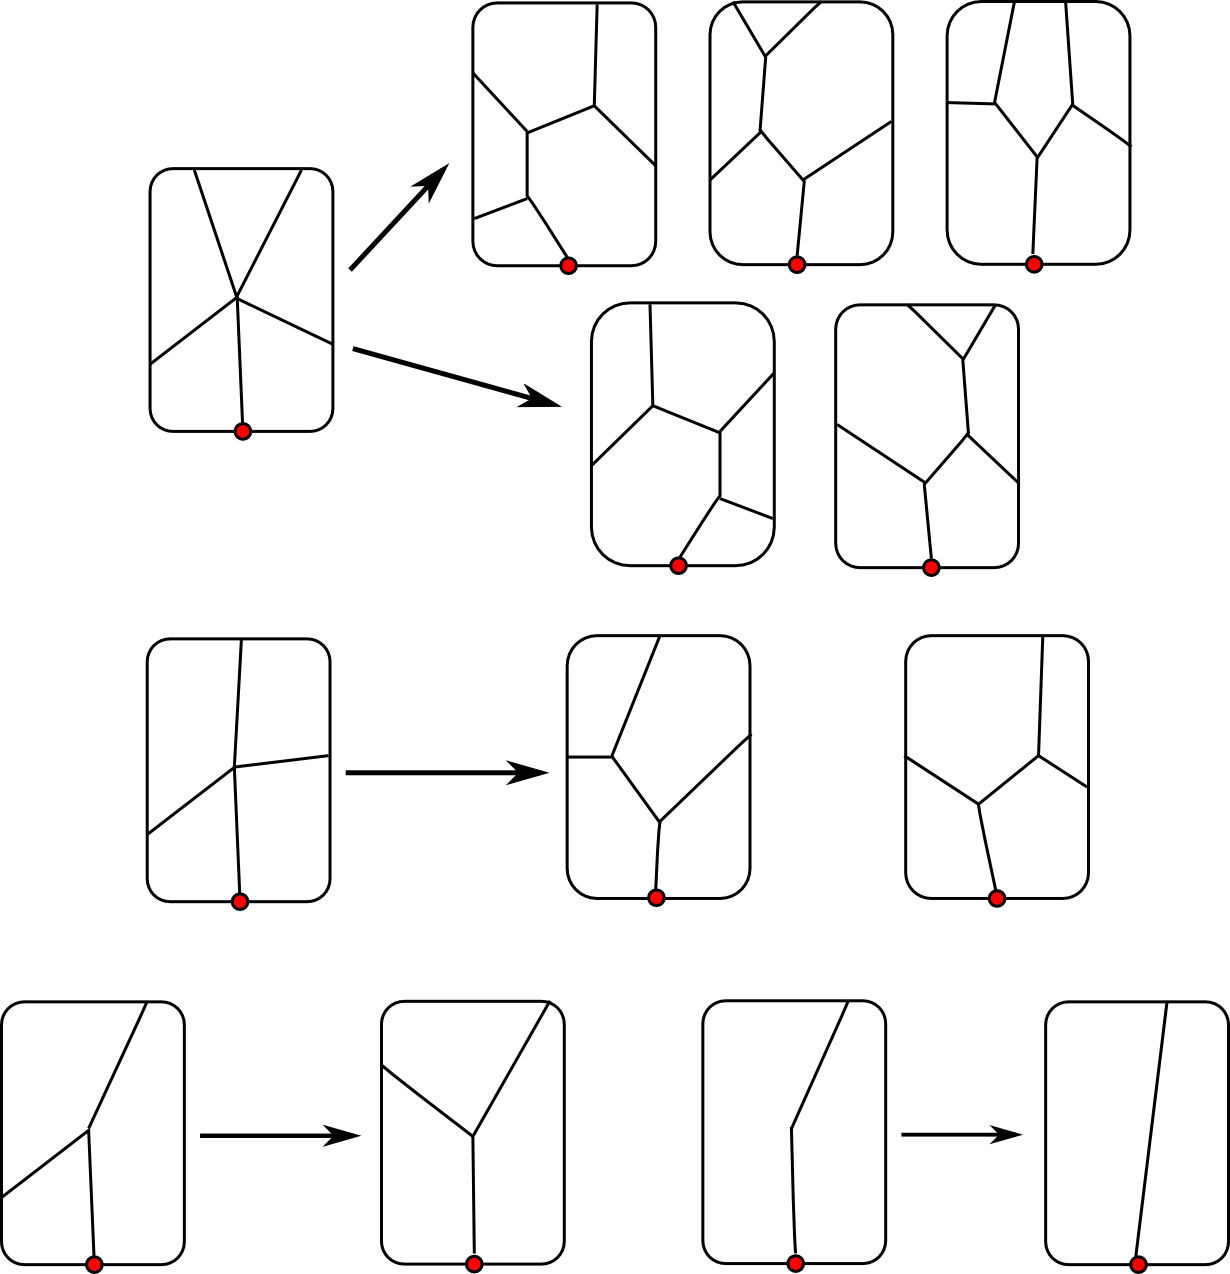
\includegraphics{graintrees.png}
\caption {\textbf{Continuation through a $k$-degree vertex. }\label{crittypes}Possible topologies of  curvature flow with $k$-ray initial conditions, with $k= 3, 4,$ and $5$. These correspond to planar rooted  trivalent tree, with the rooted vertex in each figure denoted by a dot.   } 
\end{centering}   
\end{figure}

We now combine (\ref{vertest}), (\ref{strongfaceest}), and the Euler characteristic formula to obtain
\begin{eqnarray}
V-E+F = 1-k \\
\Rightarrow F =1+\frac{E}3-\frac{2k}3\nonumber\\
\ge1+\frac{7F+3k}{6}-\frac{2k}3 \nonumber\\
\Rightarrow F\le k-6 \nonumber.
\end{eqnarray}
 We therefore search for solutions containing no faces.  Such networks are precisely trees.  Specifically, we seek trivalent trees with $k$ leaves corresponding to  edges containing $p_i$, $i = 1, \dots k$.  Since the endpoints of the leaves are fixed, the number $M_n$ of such trees is equal to the planar trivalent rooted trees of $n$ leaves, which is equal to the ${n-1}^{st}$ Catalan number $C_{n-1}$ \cite{hungerbuhler1995isomorphism}. Specifically, $M_2 = 1,M_3 = 1, M_4 = 2$, and $M_5 = 5$. 
\end{proof}
The explicit graph types are shown in Fig. \ref{crittypes}. However, regardless of topological type, flowing through a  four and five sided grain deletions gives the same topological transitions, as shown in Fig. \ref{distrules}. 


\section{PDMPs and grain coarsening}\label{applygrain}
We now demonstrate that a mean-field model of grain coarsening is a specific example of the $k$-species PDMP explored in \cite{klob2013pdmp1} .  The one parameter constants are as follows, where we index our species $i = 2, \dots, M+1$ according to the $n-gons$ (grains with $n$-sides) they describe:
 
 \begin{centering}
 \begin{tabular}{|c|c|}\hline
General Variable & Value for grain coarsening \\\hline
$M$ & $M>6$ (free parameter)\\\hline
$M_-$ & 4 \\\hline
$\beta$ & $\beta>0$ (free parameter) \\\hline
$v_i$&$i-6 $  \\\hline
$K^{(l)}$&$K^{2}=2, K^{(3)} = 3, K^{(4)}= 2, K^{(5)}= 3, K^{int} = 4$ \\\hline
\end{tabular}

\end{centering}
\vspace{10 pt}
Describing our parameters in more detail:
\begin{itemize}
\item A particle of size $a$ of species $L_n = \mathbb{R}^+, n = 2 ,\dots, M$, corresponds to an $n$-gon with area $a$. 
\item By the $n-6$ rule, the velocity $v_n(a)$ of an $n$-gon is the constant $v_n(a) \equiv n-6$. Thus, $M_- = 4$.
\item Constants $K^{(i)},K^{int}$ correspond to the number of side redistributions for each type of grain  and side deletion, e.g.  five sided grain deletions affect three grains, $K^{(5)} = 3$.     
\end{itemize}

For $n$-gon probability weights, we impose the mean-field assumption that  $n$-gon selection is proportional to $n$.  To obtain a closed system, we forbid two-sided grains to lose sides, three-sided grains to lose two sides, and $M-$sided grains to gain a side. We will not consider one-sided grains, as they are relatively rare in actual metal networks (about .1\%, see \cite{fradkov1985experimental}).  

We now give the explicit weights for $n$-gon selection in grain coarsening.  These are based on the Fradkov assumption that grains are selected based only on their side number. The weights are then
\begin{equation}
w_j^{(2)}= \begin{cases}j, & j \in \{4,\dots, M\},   \ \\
0, & j \in \{2,3\},  \ \\
\end{cases}
\end{equation}
\begin{equation}
w_j^{(3)}= \begin{cases}j, & j \in \{3,\dots, M\},   \ \\
0, & j =2,  \ \\
\end{cases}
\end{equation}
\begin{equation}
w_j^{(4)}= \begin{cases}j, & j \in \{3,\dots, M\},   \ \\
0, & j =2,  \ \\
\end{cases}
\end{equation}
\begin{equation}
w_j^{(5)}= \begin{cases}j, & j \in \{3,\dots, M-1\},   \ \\
0, & j \in\{2,M\},  \ \\
\end{cases}
\end{equation}
\begin{equation}
w_j^{int}= \begin{cases}j, & j \in \{3,\dots, M-1\},   \ \\
0, & j \in\{2,M\}.  \ \\
\end{cases}
\end{equation}

Reassignments are in accordance with  side redistribution under grain and side deletion. Recall the upper index $l= 1, \dots M_-$  in $R_{kj}^{(l)}$ refers to the side number of the deleted grain, $k= 2,\dots, M$ refers to the side number of a neighboring grain before undergoing side reassignment, and $j= 1\dots, K^{(l)}$ refers to the specific reassignment of the $j^th$ grain that is reassigned sides. Refer to Fig. \ref{distrules} for a pictorial description distribution of sides before and after grain and side deletions. Note that we disallow reassignments that create 1 and $M+1$ sided  grains. 
The explicit reassignments are then\begin{equation}
R_{kj}^{(2)}= \begin{cases}k-2, & k \in \{4,\dots, M\},j\in \{1,2\},         \\
0, & k \in \{2,3\} ,  \ \\
\end{cases}
\end{equation}
\begin{equation}
R_{kj}^{(3)}= \begin{cases}k-1, & k \in \{3,\dots ,M\},j\in \{1,2,3\}, \\
0, & k =2,  \ \\
\end{cases}
\end{equation}
\begin{equation}
R_{kj}^{(4)}= \begin{cases}k-1, & k \in \{3,\dots ,M\},j\in \{1,2\}, \\
0, & k =2,  \ \\
\end{cases}
\end{equation}
\begin{equation}
R_{kj}^{(5)}= \begin{cases}k-1, & k\in \{3, \dots,M-1\}, j \in \{1,2\},    \\
k+1, & k\in \{3 ,\dots,M-1\},j=3,\\
0, & k\in \{2 ,M\},\\
\end{cases}
\end{equation}
\begin{equation}
R_{kj}^{int}= \begin{cases}k-1, & k\in \{3, \dots,M-1\}, j \in \{1,2\},    \\
k+1, & k\in \{3 ,\dots,M-1\},j\in\{3,4\},\\
0, & k\in \{2 ,M\}.\\
\end{cases}
\end{equation}

\begin{figure}
\begin{centering}
\includegraphics{grainpic.png}
\caption{\textbf{Reassignments of sides before and after deletions.  }\label{distrules} Numbers in grains refer to side numbers.}
\end{centering}
\end{figure}
We now give an explicit form to the limiting kinetic equations of \cite{klob2013pdmp1} for grain coarsening. Assuming a continuous density of grain areas $u_k(x,t)$, we  can write a system of kinetic equations  for grains with $k$ sides:\begin{equation}\label{grainpde}
\partial_tu_{k}(x,t)+(k-6)\partial_xu_{k}(x,t) = h^{k+}_{grain}(u,t)-h_{grain}^{k-}(u,t)+h^{k+}_{side}(u,t)-h_{side}^{k-}(u,t).
\end{equation}

The four source terms of the right hand side of (\ref{grainpde}) describe, in order, addition and deletion of grains from $L_k$ due to grain deletions, and addition and deletion from $L_k$ due to side deletions.
Explicitly, they are, for $k = 2, \dots, M$,
\begin{eqnarray}
h_{grain}^{k,+}(u,t)= 8u_2(0,t)W_{k+2}^{(2)}(t)u_{k+2}(x,t)+9u_{3}(0,t)W_{k+1}^{(3)}u_{k+1}(x,t)\\+4u_{4}(0,t)W_{k+1}^{(4)}(t)u_{k+1}(x,t)+ 2u_{5}(0,t)W_{k+1}^{(5)}(t)u_{k+1}(x,t)\nonumber\\+u_{5}(0,t)W_{k-1}^{(5)}(t)u_{k-1}(x,t), \nonumber
\end{eqnarray}
\begin{eqnarray}
h_{grain}^{k,-}(u,t) = u_k(x,t)[8u_2(0,t)W_{k}^{(2)}(t)+9u_{3}(0,t)W_{k}^{(3)}(t)\\+4u_{4}(0,t)W_{k}^{(4)}(t)+3u_{5}(0,t)W_{k}^{(5)}(t)],
\nonumber
\end{eqnarray} 
\begin{equation}
h_{side}^{k,-}(u,t)= \frac{2\beta G(t)}{G_{int}(t)}[w_{k-1}^{int}u_{k-1}(x,t)+w_{k+1}^{int}u_{k+1}(x,t)],
\end{equation}
\begin{equation}
h_{side}^{k,+}(u,t)= \frac{4\beta G(t)}{G_{int}(t)}w_k^{int}u_k(x,t),
\end{equation}
for tier weights $w_i^{(l)},w_i^{int}$, total numbers $G(t),G_{int}(t)$, and species selection weight fraction $W_i^{(l)},W_i^{int}$ defined in (\ref{limeq}).
Our main result of the previous chapter is the convergence of empirical PDMPs to the weak form of (\ref{grainpde}) for absolutely continuous measures $\mu_k(t) \in \mathcal{M}(\mathbb{R}^+)$, obtained by pairing solutions $\mu_k$ with a test function $\phi \in \mathcal C$ and integrating along $\mathbb{R}^+$. The weak form of (\ref{grainpde}) is then, for  $k = 2, \dots, M$, 
 \begin{eqnarray}\label{weakgrainpde}
\langle C_k(t), \phi\rangle -  \langle C_k(0), \phi\rangle+(k-6)\int_0^t \langle C_k(s), \phi' \rangle\\= H^{k+}_{grain}(u,t)-H_{grain}^{k-}(u,t)+H^{k+}_{side}(u,t)-H_{side}^{k-}(u,t) ,\nonumber
\end{eqnarray} 
with
\begin{eqnarray}
H^{k+}_{grain}(u,t)=2\int_0^tW^{(2)}_{k+2}(s)\langle C_{k+2}(s), \phi \rangle dF_{2}(s)+\\3\int_0^tW^{(3)}_{k+1}(s)\langle C_{k+1}(s), \phi \rangle dF_{3}(s)+2\int_0^tW^{(4)}_{k+1}(s)\langle C_{k+1}(s), \phi \rangle dF_{4}(s)+ \\2\int_0^\infty W^{(5)}_{k+1}(s)\langle C_{k+1}(s), \phi \rangle+W^{(5)}_{k-1}(s)\langle C_{k-1}(s), \phi \rangle dF_5(s), \nonumber
\end{eqnarray}
\begin{eqnarray}
H_{grain}^{k,-}(u,t) =2 \int_0^t\langle C_{k}(s), \phi \rangle W^{(2)}_{k}(s)dF_2(s)\\+3\int_0^t\langle C_{k}(s), \phi \rangle W^{(3)}_{k}(s)dF_3(s)+2\int_0^t\langle C_{k}(s), \phi \rangle W^{(4)}_{k}(s)dF_4(s)\nonumber\\+3\int_0^t\langle C_{k}(s), \phi \rangle W^{(5)}_{k}(s)dF_{5}(s), \nonumber
\end{eqnarray}
\begin{equation}
H_{side}^{k,-}(u,t)= \int_0^t\frac{2\beta N(s)}{N_o(s)}[w_{k-1}^{int}\langle C_{k-1}(s), \phi \rangle+w_{k+1}^{int}\langle C_{k+1}(s), \phi \rangle]ds,
\end{equation}
\begin{equation}
H_{side}^{k,+}(u,t)= \int_0^t\frac{4\beta N(s)}{N_o(s)}w_{k}^{int}\langle C_{k}(s), \phi \rangle ds.
\end{equation}
A point of departure from the Fradkov model is the choice of side deletion parameter $\beta$.  For the PDMP model, each grain is equipped with a Poisson clock that activates with average time $\beta$.  When such a clock is activated, four grains are selected to change side number in accordance with rules for side flipping.  This differs from Fradkov's model, which assumes side deletion over grain deletion occurs at a constant ratio $\beta$.  Graphs depicting the ratio of side to grain deletions are depicted in Fig. \ref{fradrat1}-\ref{fradrat3}. .  
       


From the previous chapter, we have seen that there exists limiting subsequence that converges to a solution of (\ref{weakgrainpde}).  We now show that the solution retains several properties from the pre-limit PDMP.

\section{Properties of grain coarsening}

One advantage to the stochastic method of proving existence  of solutions to (\ref{weakgrainpde}) is that we can use properties from the finite particle PDMP model to prove, with little difficulty, that the same properties hold for the hydrodynamic limit.  Our main tool is the observation that since $\langle \mu_k^N(t),\phi\rangle \xrightarrow {l.u.} \langle \mu_k(t),\phi\rangle$ for all $\phi \in C_b(\mathbb{R}^+)$, we can choose $\phi \equiv 1$ to obtain the convergence of total numbers $g^N_k(t)\xrightarrow{l.u.} g_k(t)$.

\begin{theorem}  The following properties hold for the limiting distributions $\mu_k(t)$
\begin{enumerate}
\item (\textbf{Conservation of Polyhedral Defect}). If the initial average side number for grains is 6, it remains so:
\begin{equation}
\sum_{k = 2}^M(k-6)g_{k}^0= 0 \quad \Rightarrow \quad P(t):=\sum_{k = 2}^M(k-6)g_k(t)= 0.
\end{equation}
\item (\textbf{No runoff at infinity}).  All loss of total number occurs from boundary events, or
\begin{equation}
N(t) := \sum_{k =2}^M g_k(t) =  \sum_{k = 2}^M g_{k}^0-\sum_{i = 2}^5 F_i(t).
\end{equation}
\item (\textbf{Decreasing densities}).  The total number is decreasing in time:
\begin{equation}
N(t)\le N(s) \quad \hbox{ for } t\ge s.
\end{equation}
\end{enumerate}
\end{theorem}
\begin{proof}
Suppose we have a limiting initial measure $\mu_k^0$ with zero polyhedral defect. For $i \in \mathbb N$, let $\mu_k^{N_i,0}\in \mathcal M(\mathbb R^+)$  be a sequence of initial empirical distributions of particles with zero polyhedral defect, satisfying $\mu_k^{N_i,0} \rightarrow \mu_k^0 $ in $\mathcal M(\mathbb{R}^+)$. Constructing such a sequence is always possible. To see this, choose integers $N_i \rightarrow \infty$  ,where $N_i= N_i^2+\dots+N_i^M$ , $\sum_{k = 2}^M (k-6)N_i^k = 0 $, and $N_i^k/\sum_j N_i^j \rightarrow g_{i,0}$. For each $n$-gon in $L_n$, randomly select $N_i^k$ particles with respect to the distribution $\mu_k^0$.  By the Glivenko-Cantelli theorem, with probability one the empirical distributions  $\mu_k^{N_i,0}$ will converge  to $\mu_k^0$ in $\mathcal M(\mathbb{R}^+)$.  
 
For the empirical measures $\mu^{N_i,0}(t)$, it is straightforward to see conservation of polyhedral defect.  This is because transport of grains does not change a grain's side number, and one can check that any critical event has a net zero change in polyhedral defect. Thus  
\begin{equation}
P^{N_i}(t) :=\sum_{k = 2}^M(k-6)g_k^{N_i}(t)= 0.     
\end{equation}
Since $g_k$ is the local uniform limit of $g_k^{N_i}(t)$, we obtain property (1).

For property (2), we again choose a sequence of empirical initial measures $\mu_k^{N_,0} \rightarrow \mu_k^0 $ in $\mathcal M(\mathbb{R}^+)$, this time with no further qualifications. For the empirical densities, we have 
\begin{equation}\label{totalmass}
\sum_{k =2}^M g_k^N(t) =  \sum_{k = 2}^M g_{k,0}^{N}-\sum_{i = 2}^5 F_i^N(t). \end{equation}
In the previous chapter we've shown that $F_i^N(t) \xrightarrow{l.u.} F_i(t)$, so taking the local uniform limit proves (2).  Statement (3) then follows immediately from (\ref{totalmass}), as the cumulative distributions $F_i$ are increasing.     
\end{proof}


Our next task is to show that our system conserves area, which is a consequence of conservation of polyhedral defect.  In this case, we'll  use the weak form of the limiting equations.  Here, we denote the identity function $id: x \mapsto x$.     
\begin{theorem}(\textbf{Conservation of area}).  For initial distributions which satisfy
\begin{equation}
\sum_{k = 2}^M\langle \mu_k^0,id\rangle< \infty, \quad P(0) = 0, 
\end{equation} 
we have 
\begin{equation}
\sum_{k = 2}^M\langle \mu_k(t),id\rangle = \sum_{k = 2}^M\langle \mu_k^0,id\rangle
\end{equation}
\end{theorem}
\begin{proof}  For $r,j>0$, we use functions $\phi^{r,j}:\mathbb{R}^+ \rightarrow \mathbb{R}^+$ defined by
\begin{equation}
\phi^{r,j}(x) = \begin{cases}x & x<r \\
\psi^{j}(x-r)+r & x \in [r,r+\frac 1j] \\
r  \ & x > r+\frac 1j,
\end{cases}
\end{equation}
where $\psi^j:[0,\frac 1j]\rightarrow \mathbb{R}^+$ is a $C^1(\mathbb{R}^+)$ function with $\psi'(0) = 1$ and $\psi'(\frac1j) = 0$, so that $\phi^{r,j}\in \mathcal C$.  If we sum (\ref{grainpde})  over grain classes, a simple  (though lengthy) calculation shows that
\begin{equation}
\sum_{k = 2}^MH^{k+}_{grain}(u,t)-H_{grain}^{k-}(u,t)+H^{k+}_{side}(u,t)-H_{side}^{k-}(u,t)= 0.
\end{equation}
Intuitively, this identity simply states that critical events change side numbers of grains, but not their areas.  We are left with the relation
\begin{equation}\label{finitearea}
\sum_{k = 2}^M\langle \mu_k(t), \phi^{r,j}\rangle =  \sum_{k = 2}^M\langle \mu_k(0), \phi^{r,j}\rangle-\sum_{k = 2}^M(k-6)\int_0^t \langle \mu_k(s), (\phi^{r,j})' \rangle.
\end{equation}
Notice, however, that 
\begin{equation}
\langle \mu_k(s), (\phi^{r,j})' \rangle= \mu_k(s)([0,r))+\int_0^{\frac 1j}\psi^j d\mu_k(s) \rightarrow g_k(s) \hbox{ as } r,j\rightarrow \infty.
\end{equation}  
This implies that taking the limit as $j,r\rightarrow \infty$ in (\ref{finitearea}) gives
\begin{equation}
 \sum_{k = 2}^M\langle \mu_k(t), id\rangle =  \sum_{k = 2}^M\langle \mu_k(0), id\rangle-\int_0^t P(s)ds.
\end{equation}
Our theorem then follows from conservation of polyhedral defect.
\end{proof}

\section{Computations}\label{computations}
Simulations for PDMP grain coarsening were performed in Matlab. Grains over several different initial configurations and $\beta$ parameters were tested. Illustrations, unless otherwise noted, are with $N= 9\times 10^4$ initial grains with a maximum of 20 sides. \textbf{Uniform initial distributions} have $10^4$ $n$-gons, for $n=2, \dots, 10$, distributed uniformly in $[0,1]$.   At time  $t= 5$ the number of grains drops an order of magnitude (see figure \ref{grainnumber}).  We observe the following:
\subsection*{Mean area growth}
Simulations of grain networks which directly approximate mean curvature flow suggest that the average grain area grows linearly.   (see, \cite{elsey2009diffusion,anderson1984computer,wakai2000three}, for instance). In our simulations, the plot the average area $\langle A_\beta(t)\rangle$ at time $t$ for the grain coarsening PDMP with varying Poisson parameters $\beta$. For small values of $\beta$,   $\langle A_\beta(t)\rangle$ is approximately linear (see Fig. \ref{av1},\ref{av2}).  The same behavior holds for average area of grains with $k$ sides, $k = 1, \dots, M$. For larger values of $\beta$, coarsening becomes convex (Fig. \ref{av3}).

\subsection*{Distribution of $n$-gons} For low values of $\beta$, the distribution of $n$-gons is approximately stationary (see Fig. \ref{sidedist1}) .  However, as $\beta$ increases, distributions of  $n$-gons $n= 3, \dots, 9$ become more uniform  as time increases (Fig. \ref{sidedist3}). This is similar to the numerical experiments of Fradkov \cite{fra881}.   Plots of $n$-gon densities for $\beta = 0$ and the Kinderlehrer model described in \cite{kin06} for stationary densities (time $t= 5$ for both models) shows a similarity of  statistics (see Fig. \ref{kindcompare}).    

 \subsection*{Grain densities and diffusion} In Fig. \ref{tierdens1}-\ref{tierdens9}, we plot histograms for grain densities of 4, 6, and 8 sides under $\beta$ values of .01, .1, and 1.  Each bar represent a bin of 40 grains. From grain deletions, the number of bars decreases, corresponding to a decrease in number for increasing time.  The densities for all $n$-gons drift to the right with time (see Fig. \ref{averagewhole}).  The parameter $\beta$ appears to play a diffusing role, as larger $\beta$ also correspond to increased variance.  
   
\subsection*{Side to grain deletion ratio} As observed in Section \ref{applygrain}, the PDMP model differs from the Fradkov model in its choice of parameter $\beta$. Thus, we will denote $\gamma_{\beta}(t)$ as the (time dependent) ratio of side deletions to grain deletions. For a uniform initial distribution,  under differing $\beta$,  $\gamma_{\beta}(t)$ exhibits similar concave profiles   (see Fig. \ref{fradrat1}-\ref{fradrat3}).









\section{Remarks}


A major advantage to viewing grain growth statistics as approximations of a hydrodynamic limit  is the relative ease of implementing simulations.  As we have seen, we can immediately raise several conjectures about grain behavior.  For example, for $\beta = 0$, does there exist a stable attractor for the distribution of $n$-gon densities?  Several details of the limiting densities make this question difficult.  First, individual $n$-gon densities do not have stable attractors.  Also, we still have yet to establish existence for an infinite time, which would be central in an asymptotic analysis.  Such long time existence was established for the Fradkov system in \cite{henseler2008kinetic}, but the existence of universal attractors in this model remains unanswered.        

   The role of the flipping parameter $\beta$ plays an interesting role in altering grain statistics. The general trend noted in simulations is that $\beta$ tends to act as a diffusion agent between $n$-gons. The rule for side flipping is similar to the particle transfer rule in the following model, as described in \cite{bruus2008theoretical}.  Here, we are approximating the dispersal of a fluid plug with initial density $u_{0}(x,y)$ in a carrier fluid. If the fluid has a vertical velocity profile of $V(y)$, the governing equations for the evolving density $u(x,y,t)$ have the form
\begin{eqnarray}
u_t-V(y)u_{x} = \frac{\alpha}2 u_{yy}\\
u(x,y,0) = u_0(x,y). \nonumber
\end{eqnarray}
The factor $\alpha$ is the diffusivity factor for the plug.  Taken as a $k$-species PDMP, we can approximate the domain carrier fluid by a large number of horizontal tiers, and then approximately the fluid plug as particles traveling on these tiers with velocity $V(y^*)$ for a tier located at $y = y^*$.  This model has no particle deletions (the fluid is conserved), but each particle is equipped with a Poisson clock of parameter $\alpha$, that when set, transfers a particle  to the next highest species with probability 1/2, and to the next lowest species with probability 1/2.  This, rule, however, is roughly the same as side flipping. In both models, for $n$ particles that are selected in an intermediate species, roughly $n/2$ will transfer upwards by one species, and $n/2$ will lower by a species. Thus, it is reasonable to expect the $\beta$ parameter in grain coarsening to act in a similar manner as the diffusion parameter $\alpha$ for the fluid plug. This is, of course, not precise, as we have not actually shown the right scaling of vertical species interspacing for the fluid plug, nor have we considered how grain deletions may interact with  diffusion due to side deletion.
\begin{figure}
\hspace{130pt}\includegraphics[width=.3\textwidth]{fluidpic.png} 
\caption{\textbf{Dispersal of a fluid plug.}  A carrier fluid   is approximated by horizontal tiers, and a fluid plug (the inner region of the figure) is approximated by particles (denoted by dots) which travel horizontally on tiers corresponding to the vertical velocity profile $V(y)$.}
\end{figure}

 
\clearpage{}

\begin{figure}
   \begin{centering}     
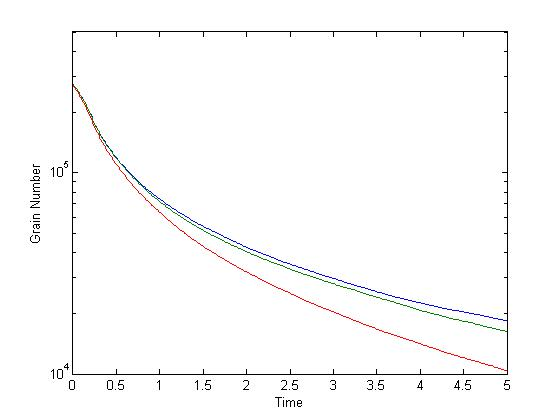
\includegraphics[width=.5\textwidth]{grainnumber.jpg}
        \caption{\textbf{Grain number} $N(t)$.}\label{grainnumber}
        \end{centering}
  \end{figure}

 \begin{figure}
 \begin{centering}
  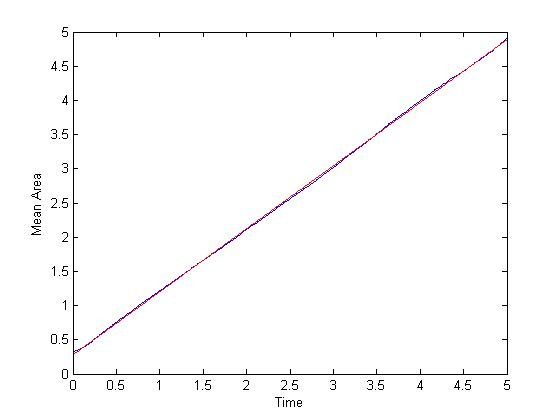
\includegraphics[width=.5\textwidth]{meanregareazero.jpg}
\caption{\textbf{Mean area of grains with $\beta = .01$} Mean area is plotted with line of best fit $y_1 = .2806+.9214x$  (the lines are indistinguishable). The correlation between average area and $y_1$ is $r^2= .9998$. }\label{av1}
\end{centering}
\end{figure}

\begin{figure}
  \begin{centering}
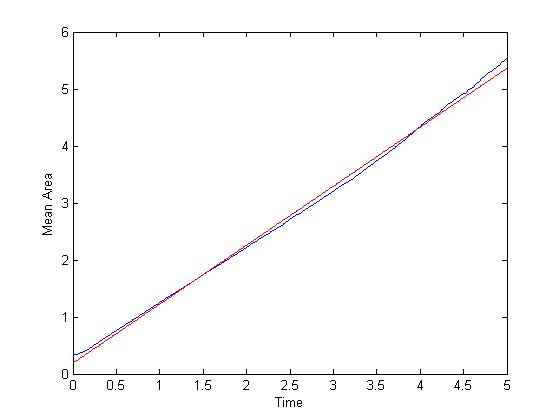
\includegraphics[width=.5\textwidth]{meanregareatenth.jpg}
\caption{\textbf{Mean area of grains with $\beta = .1$} Mean area is plotted with line of best fit $y_1 = .1909+1.0347x$   (the lines are almost indistinguishable). The correlation between average area and $y_1$ is $r^2= .9979$. }\label{av2}
\end{centering}
\end{figure}

\begin{figure}
  \begin{centering}
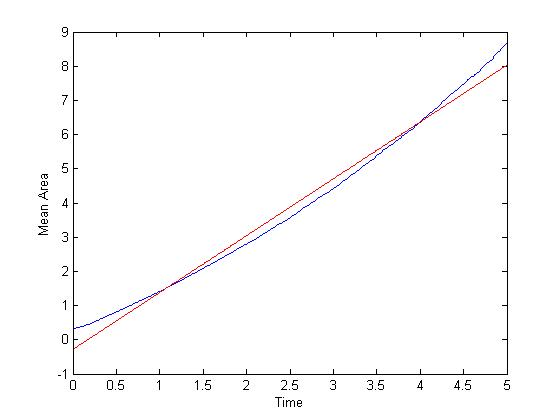
\includegraphics[width=.5\textwidth]{meanregareaone.jpg}
\caption{\textbf{Mean area of grains with $\beta = 1.$} Mean area is plotted with line of best fit $y_1 = -.2796+1.6624x$   (mean area is convex). The correlation between average area and $y_1$ is $r^2= .9881$. }\label{av3}
\end{centering}
\end{figure}



\begin{figure}
\begin{centering}
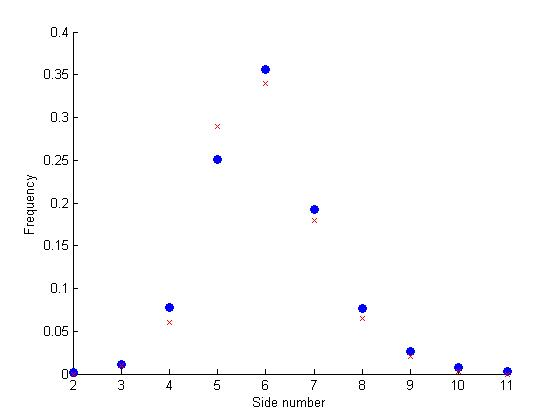
\includegraphics[width=.5\textwidth]{kindocompare.jpg}
\caption{Comparison of side number frequency between grain coarsening PDMP (dots) at $\beta= 1$ and the Kinderlehrer model (crosses) at $t= 5$.}\label{kindcompare}
\end{centering}
\end{figure}

\begin{figure}
        \begin{centering}
        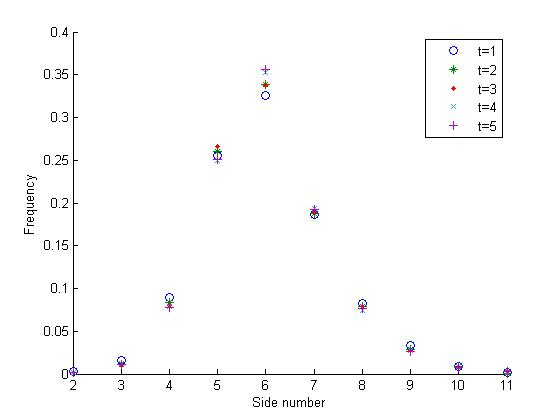
\includegraphics[width=.5\textwidth]{classdistzero.jpg}
        \caption{Frequency of side number for $\beta= .01$ for various times.}\label{sidedist1}
\end{centering}
\end{figure}

\begin{figure}
        \begin{centering}
        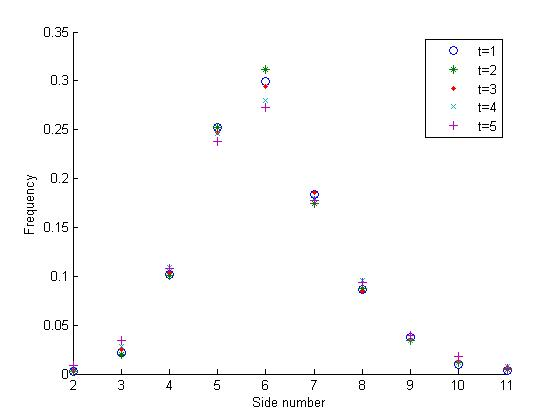
\includegraphics[width=.5\textwidth]{classdisttenth.jpg}
        \caption{Frequency of side number for $\beta= .1$ for various times.}
\end{centering}
\end{figure}

\begin{figure}
        \begin{centering}
        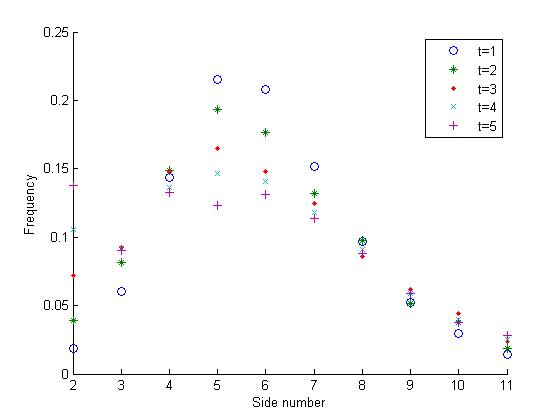
\includegraphics[width=.5\textwidth]{classdistone.jpg}
        \caption{Frequency of side number for $\beta= 1$ for various times.}\label{sidedist3}
\end{centering}
\end{figure}
        
        
        
        

 




       
        
        
        





        
        
       


\begin{figure}
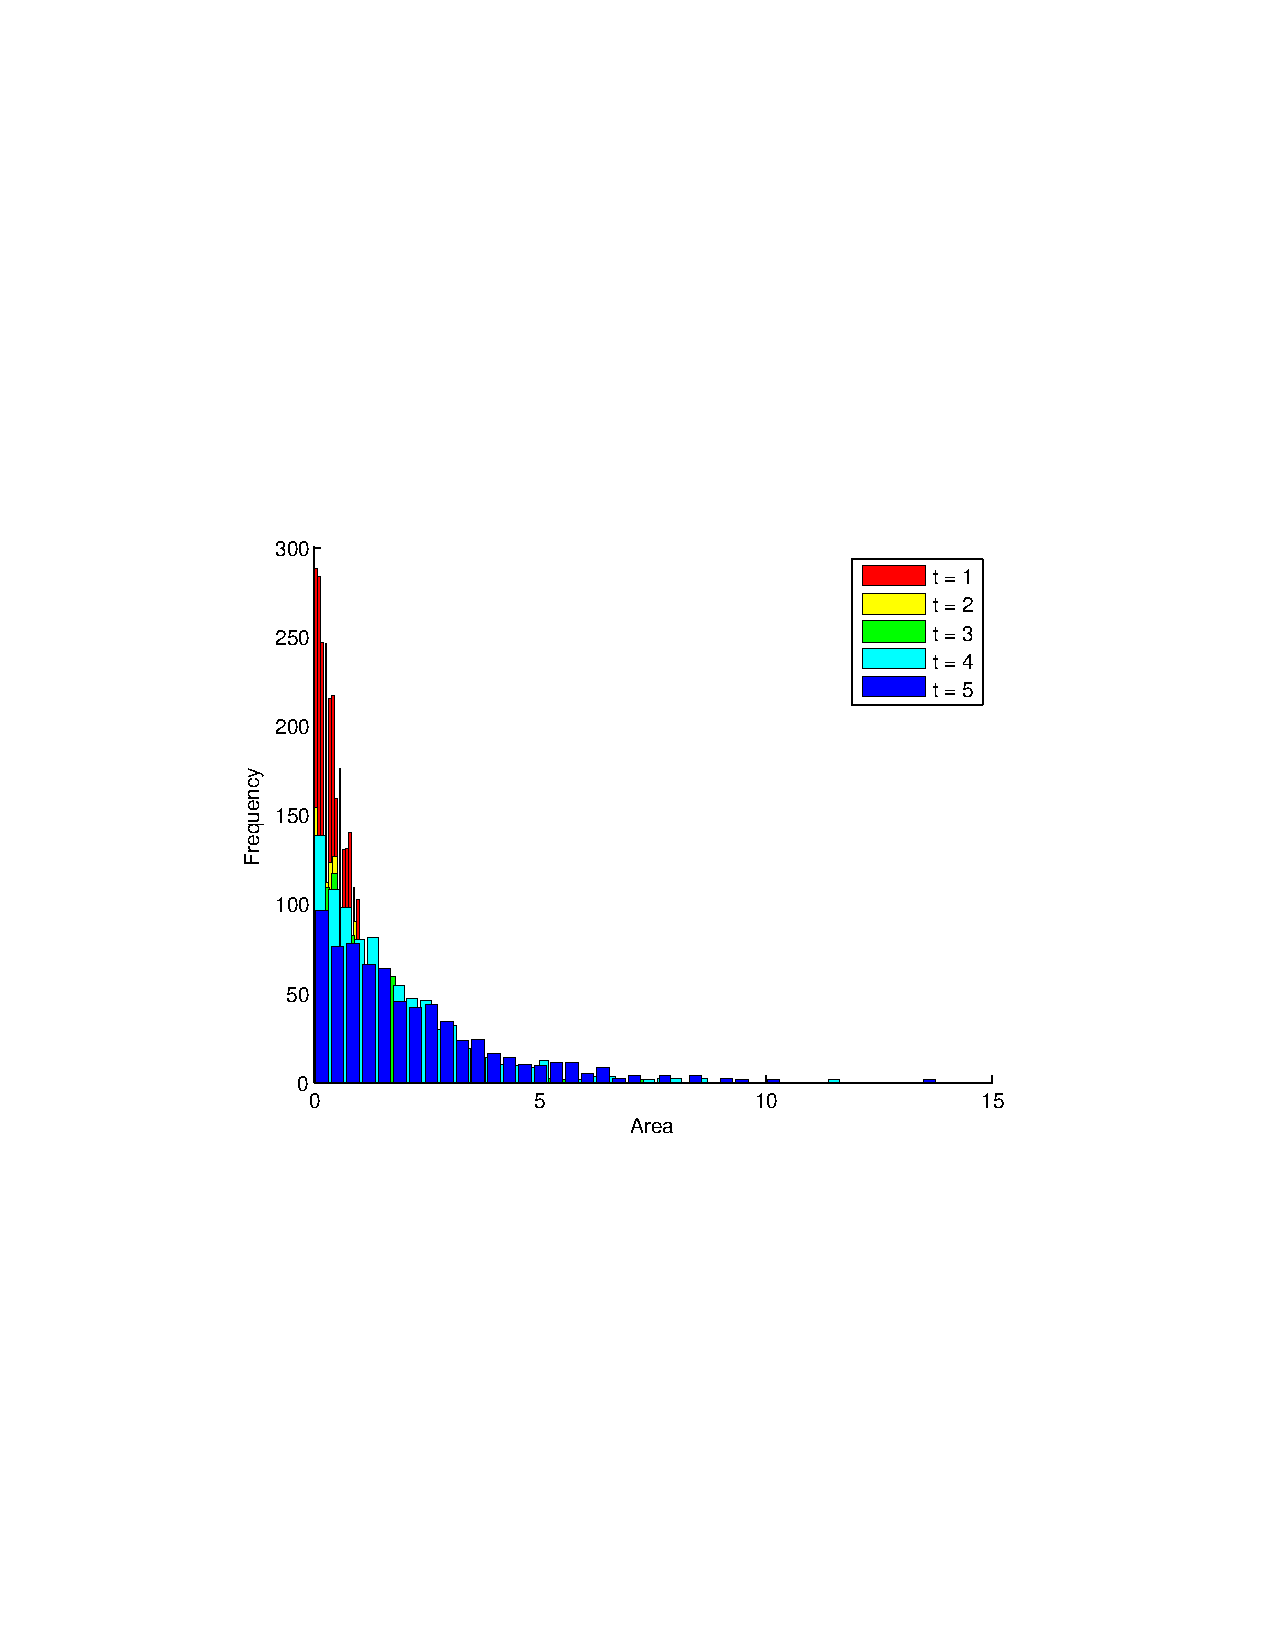
\includegraphics[width=\textwidth]{histbetazerotier4.pdf}
\vspace{-130pt}
\caption{Histograms of four-sided grain densities at $\beta = .01$.}\label{tierdens1}
\end{figure}

\begin{figure}
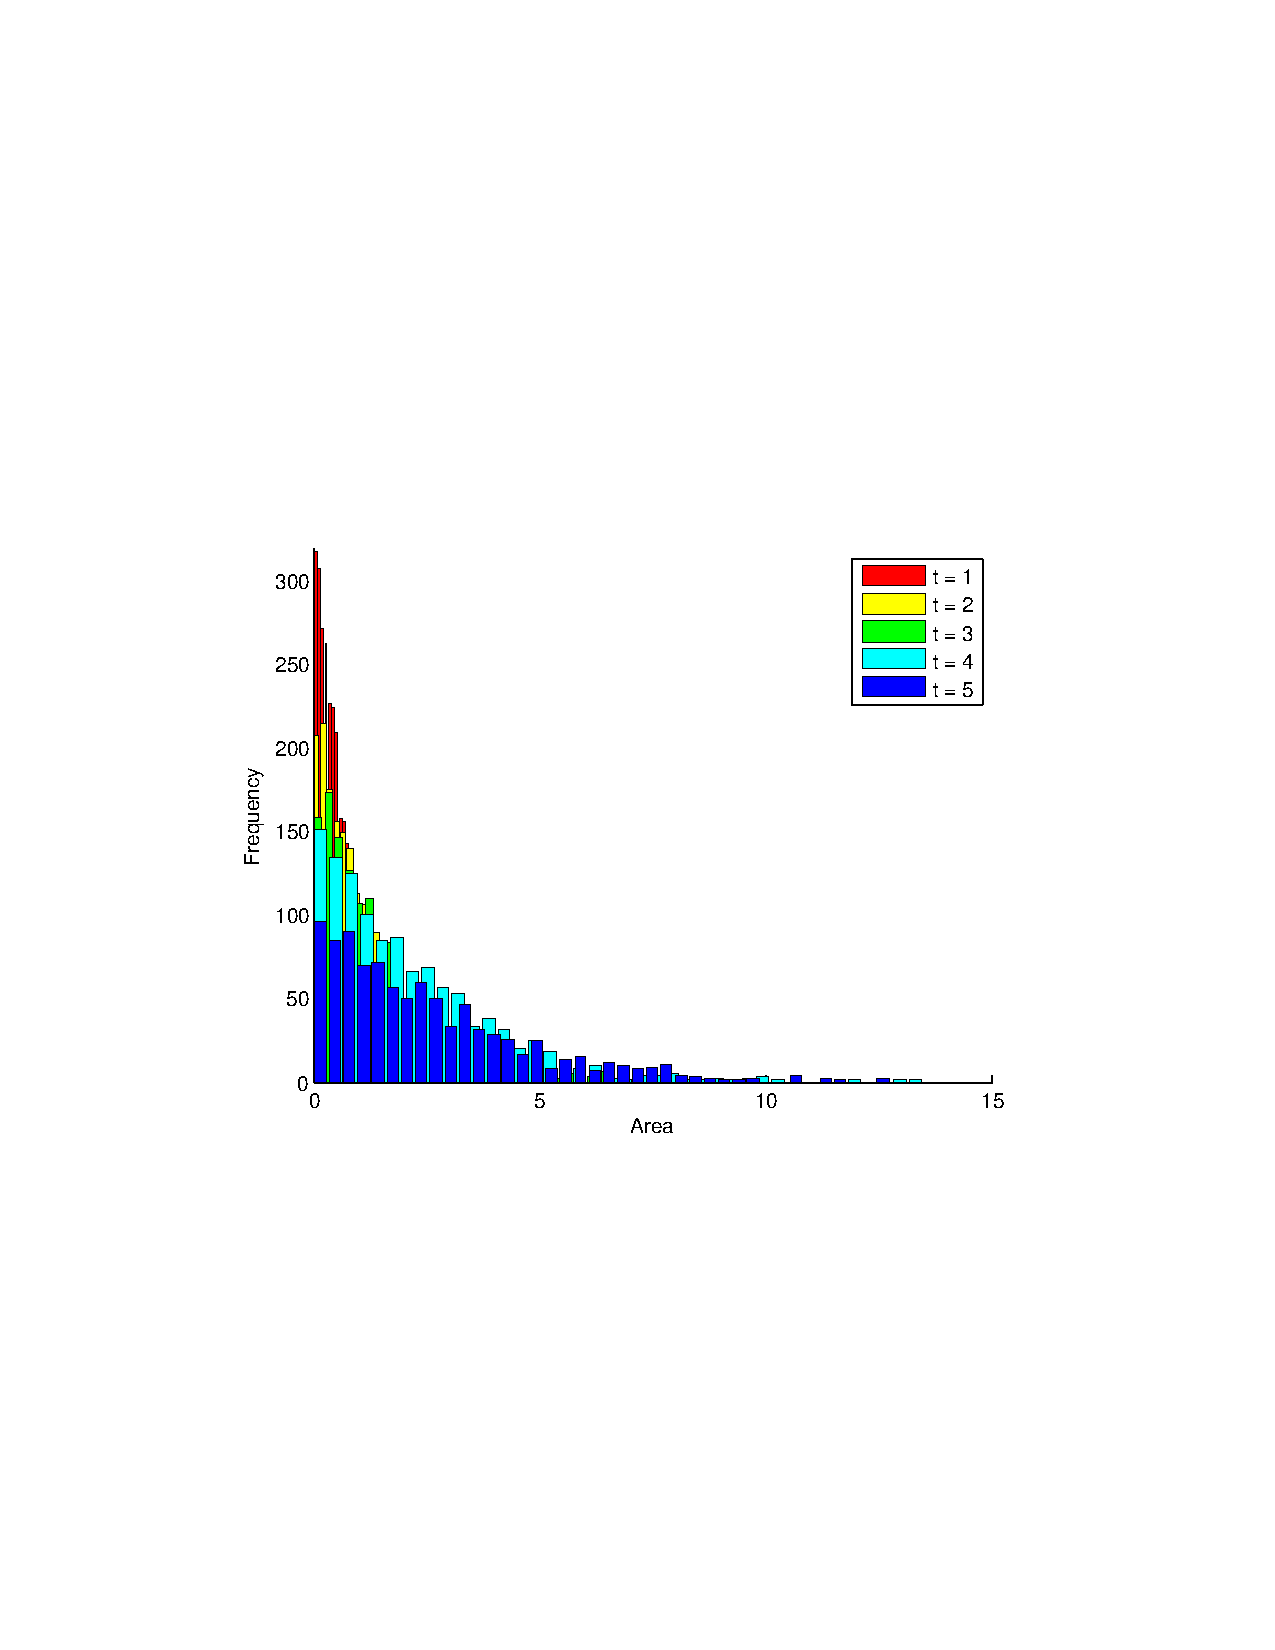
\includegraphics[width=\textwidth]{histbetatenthtier4.pdf}
\vspace{-130pt}
\caption{Histograms of four-sided grain densities at $\beta = .1$.}
\end{figure}

\begin{figure}
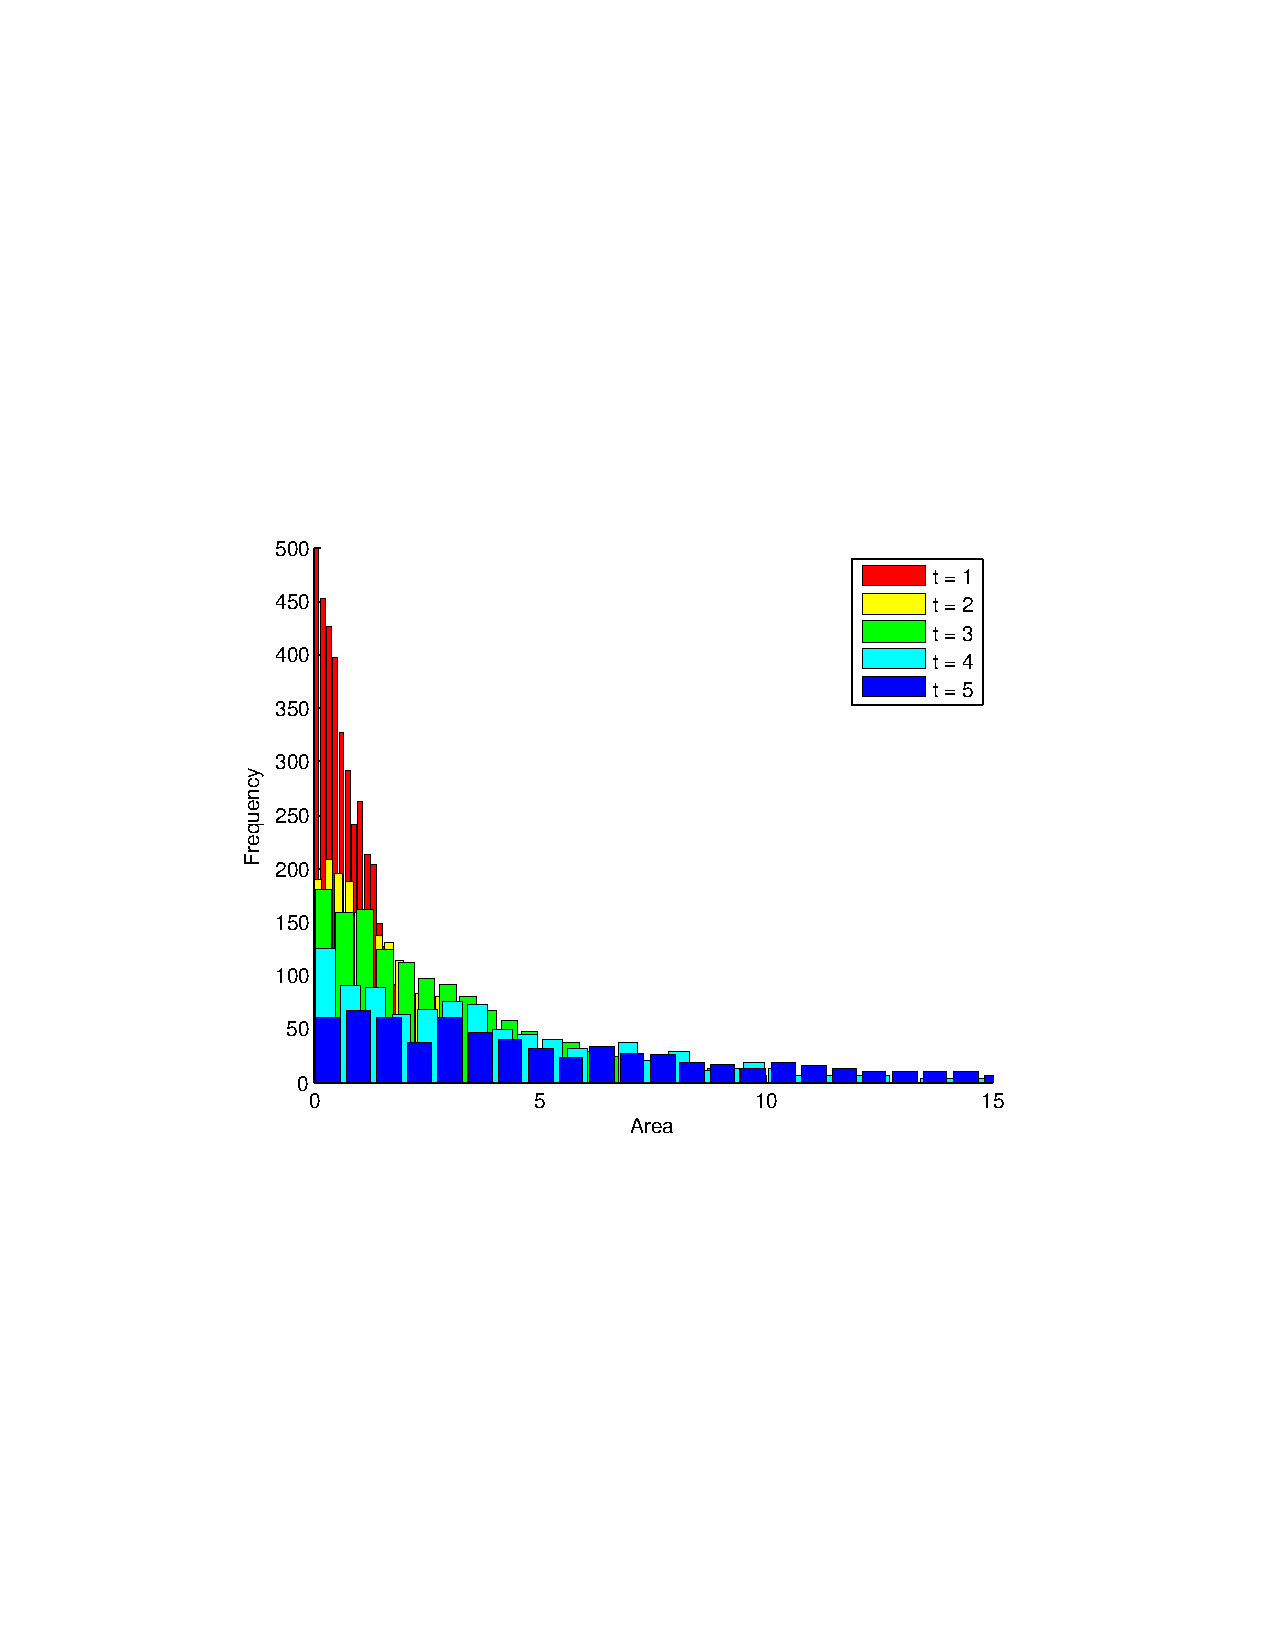
\includegraphics[width=\textwidth]{histbetaonetier4.pdf}
\vspace{-130pt}
\caption{Histograms of four-sided grain densities at $\beta = 1$.}
\end{figure}

\begin{figure}
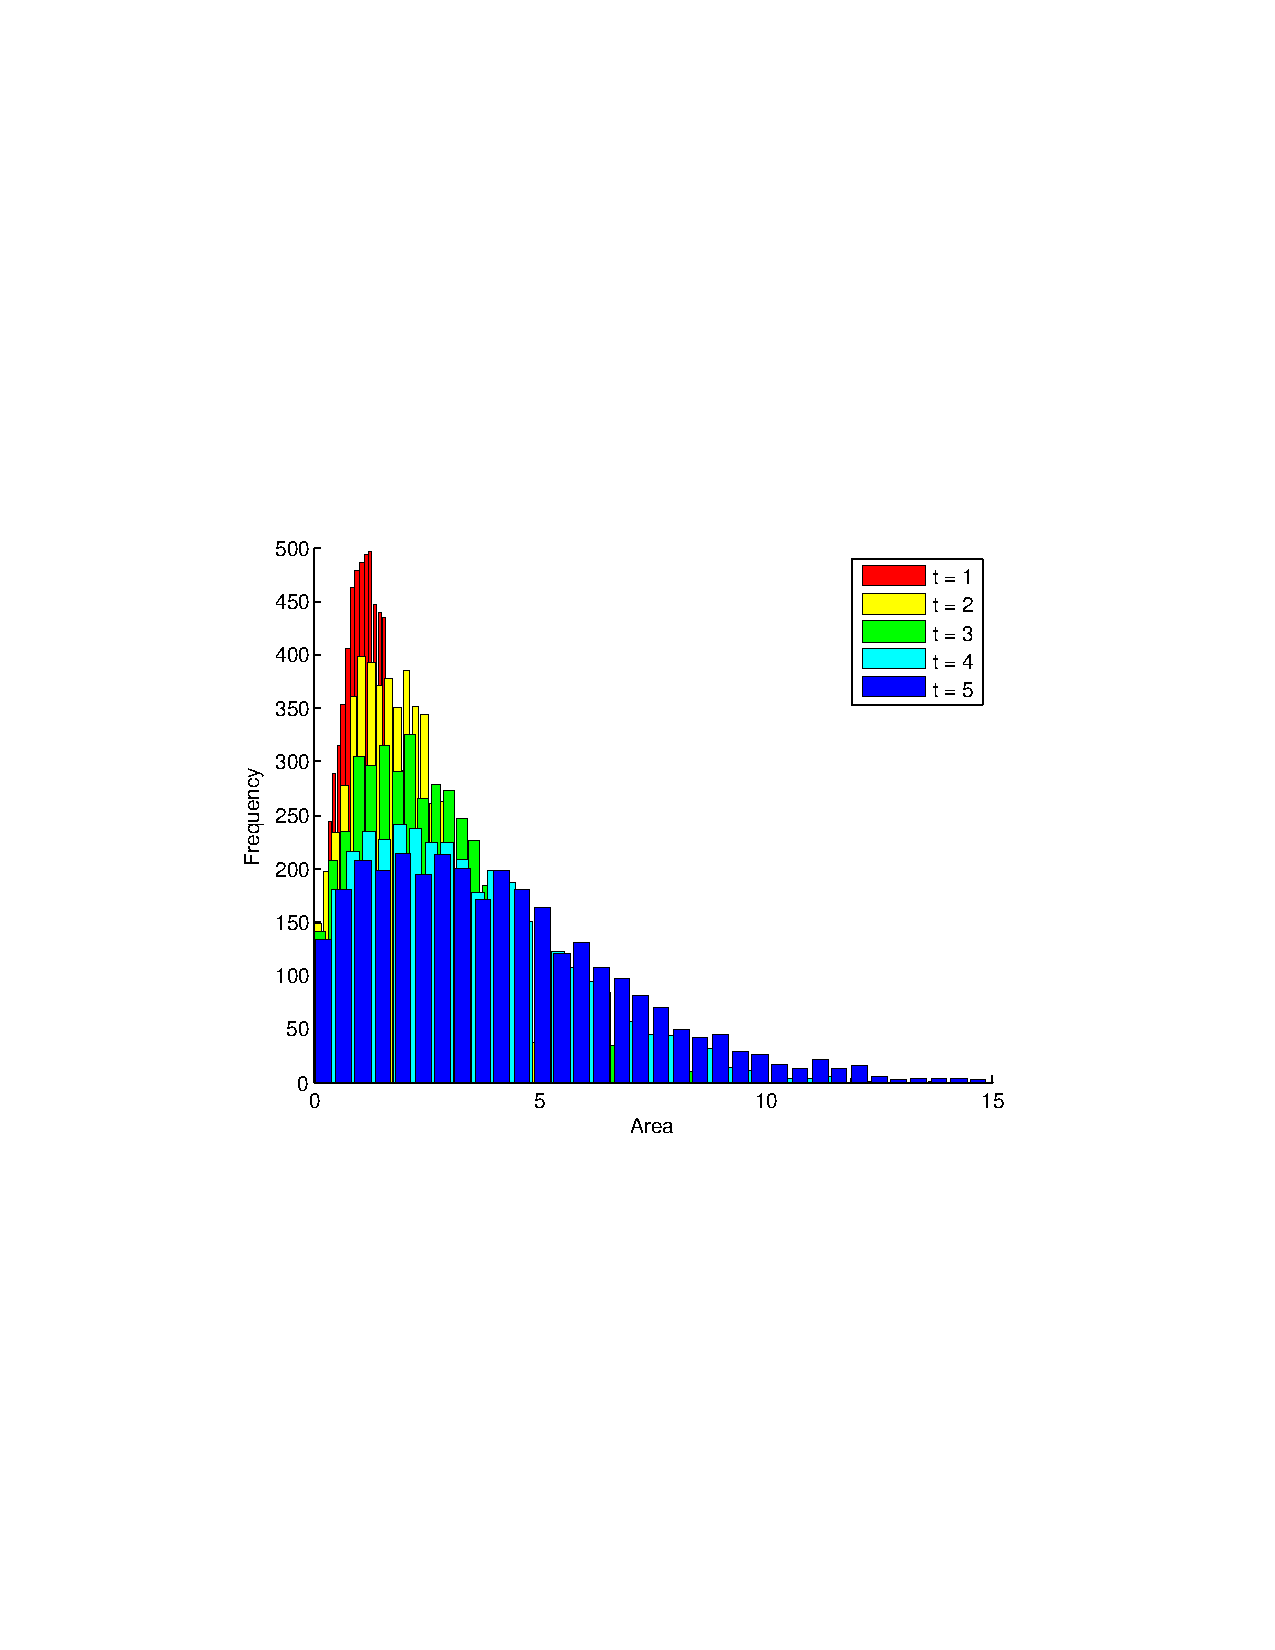
\includegraphics[width=\textwidth]{histbetazerotier6.pdf}
\vspace{-130pt}
\caption{Histograms of six-sided grain densities at $\beta = .01.$}
\end{figure}

\begin{figure}
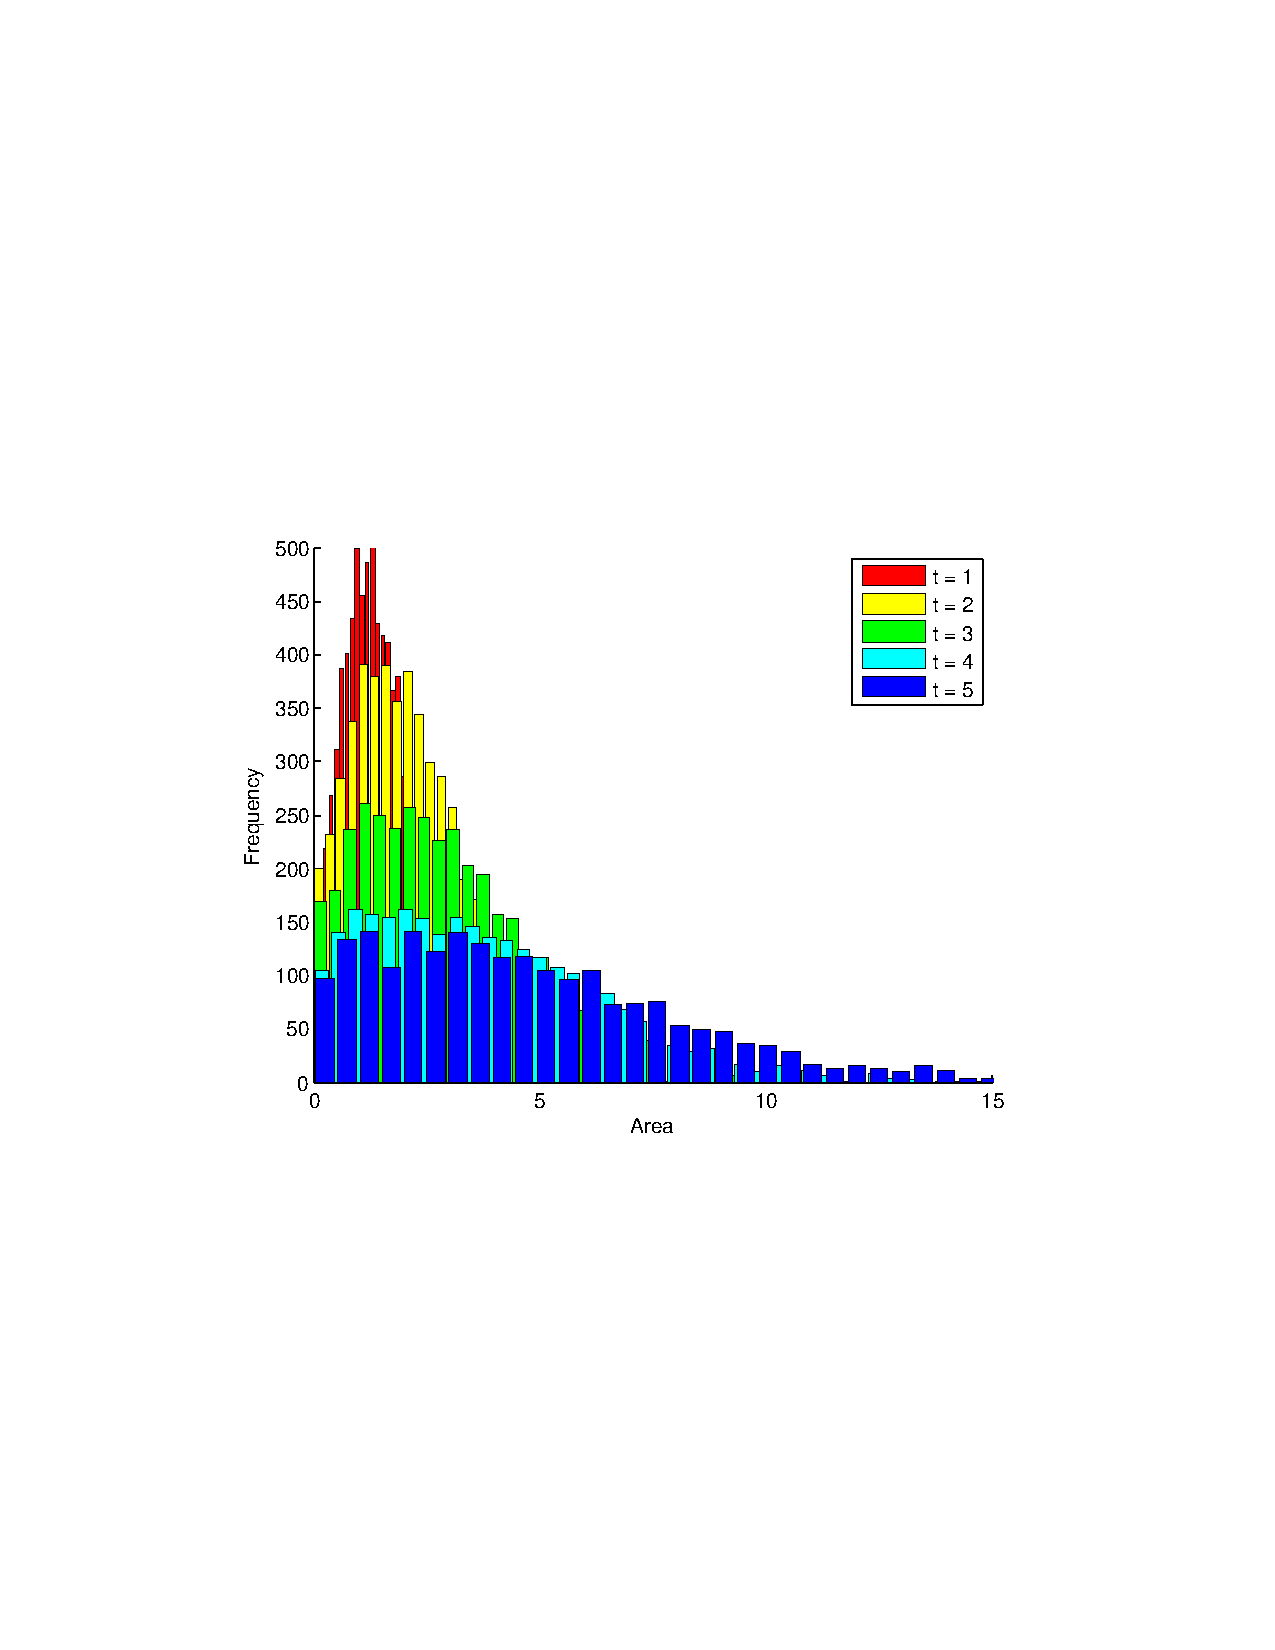
\includegraphics[width=\textwidth]{histbetatenthtier6.pdf}
\vspace{-130pt}
\caption{Histograms of six-sided grain densities at $\beta = .1$.}
\end{figure}

\begin{figure}
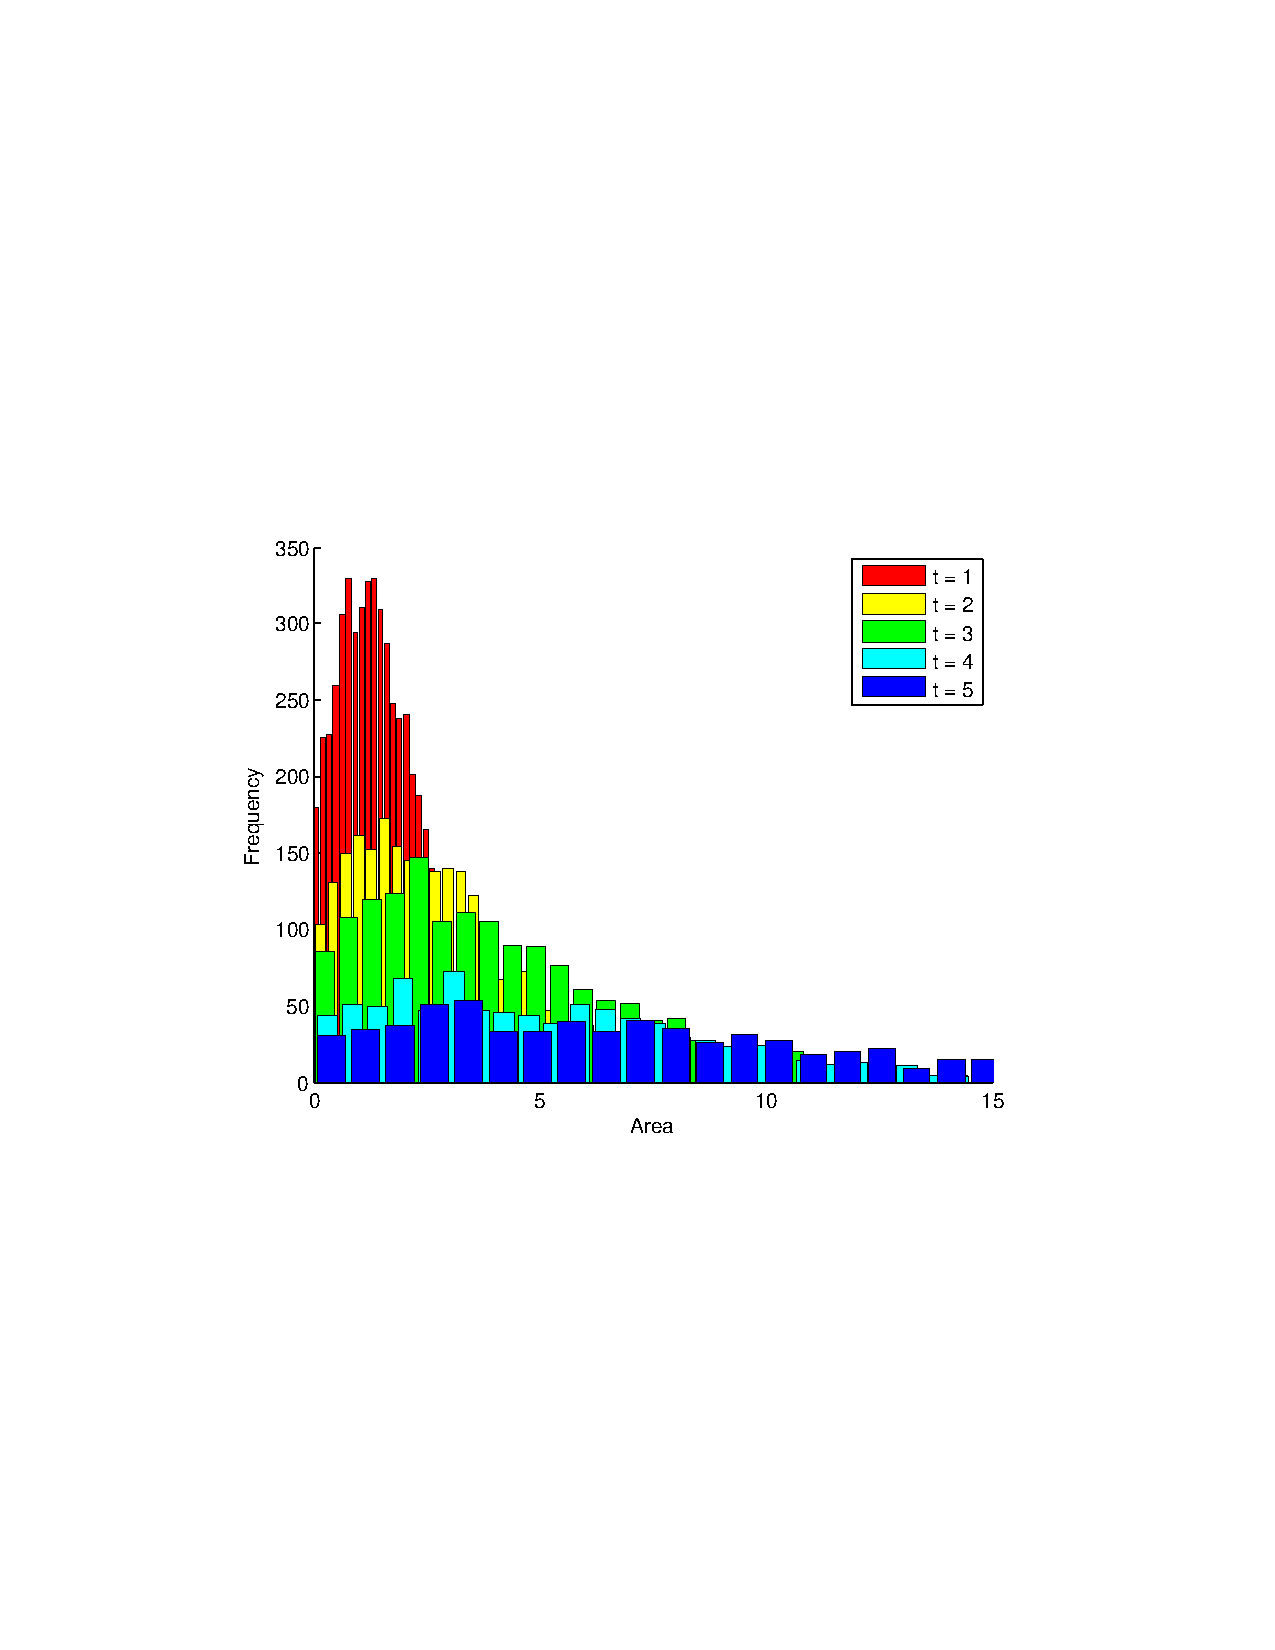
\includegraphics[width=\textwidth]{histbetaonetier6.pdf}
\vspace{-130pt}
\caption{Histograms of six-sided grain densities at $\beta = 1$.}
\end{figure}

\clearpage{}


\begin{figure}
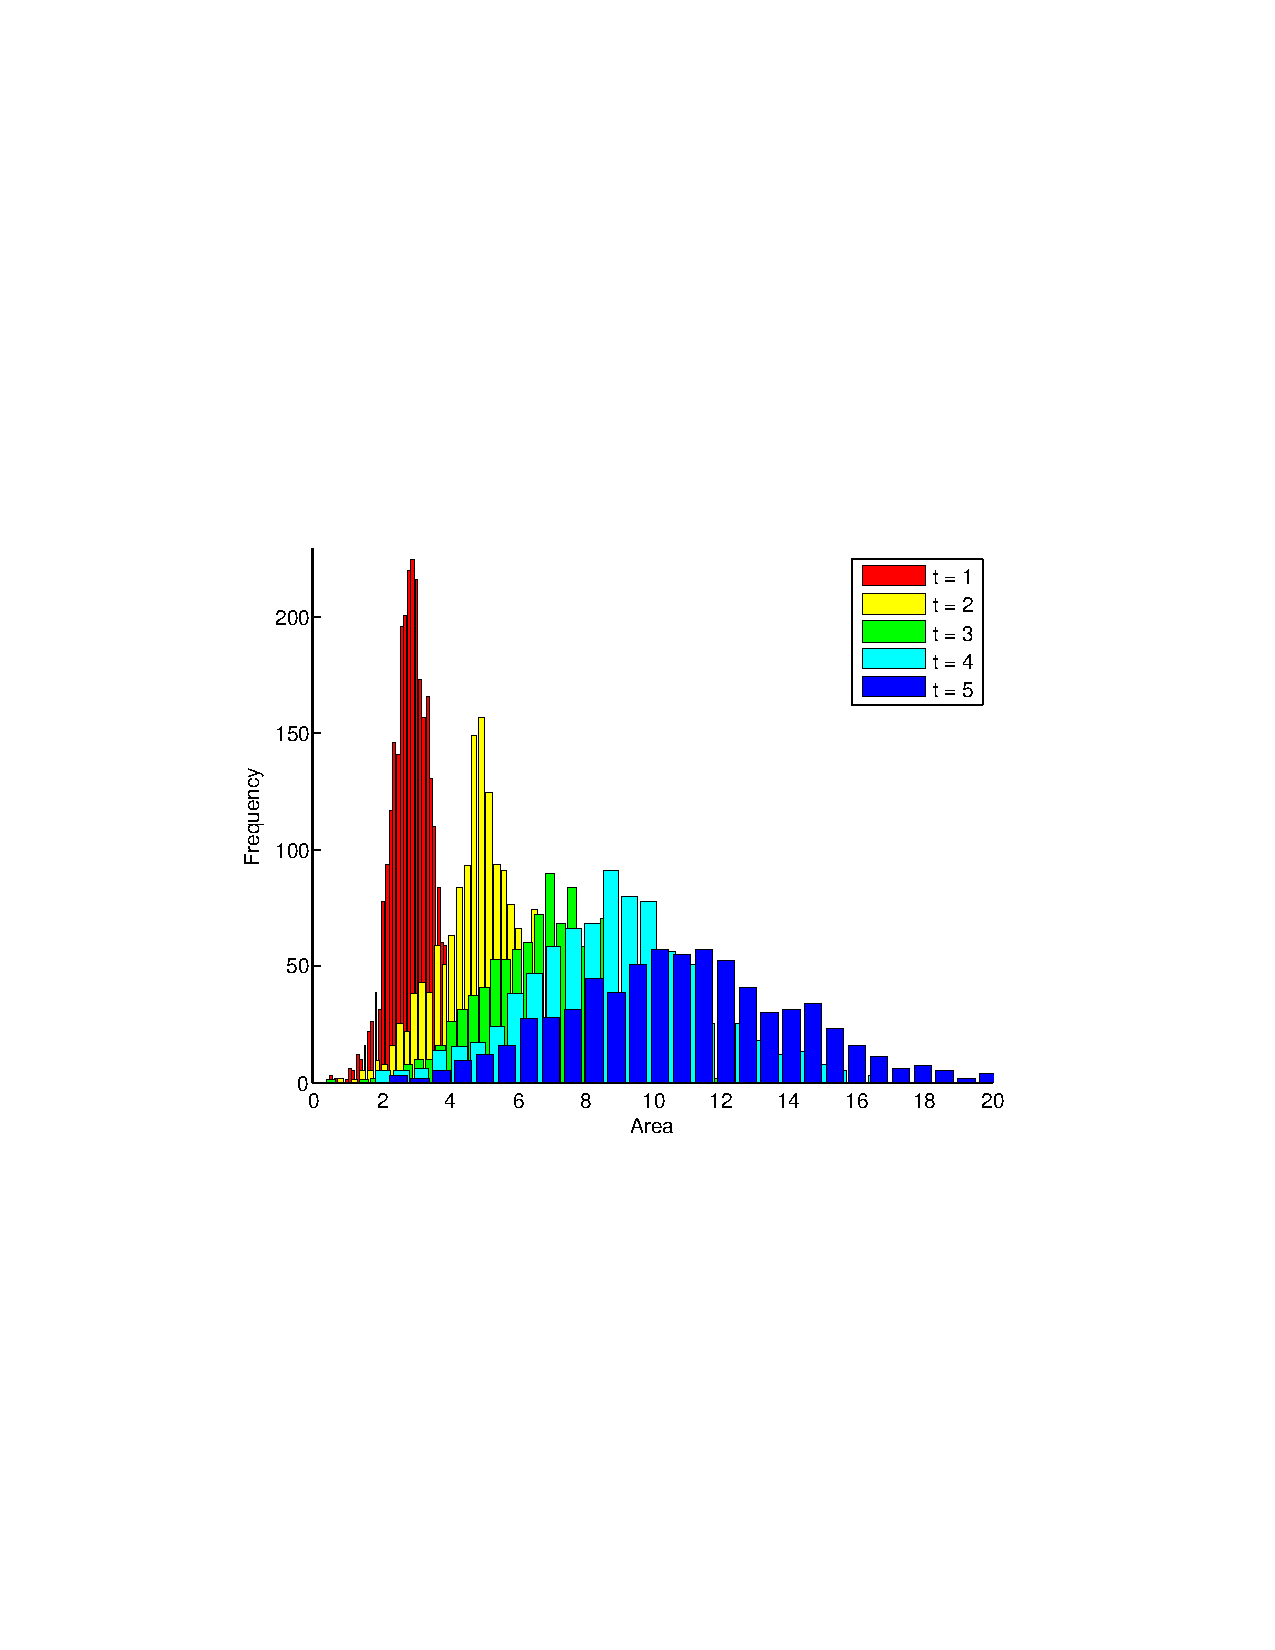
\includegraphics[width=\textwidth]{histbetazerotier8.pdf}
\vspace{-130pt}
\caption{Histograms of eight-sided grain densities at $\beta = .01$.}
\end{figure}

\clearpage{}
\begin{figure}
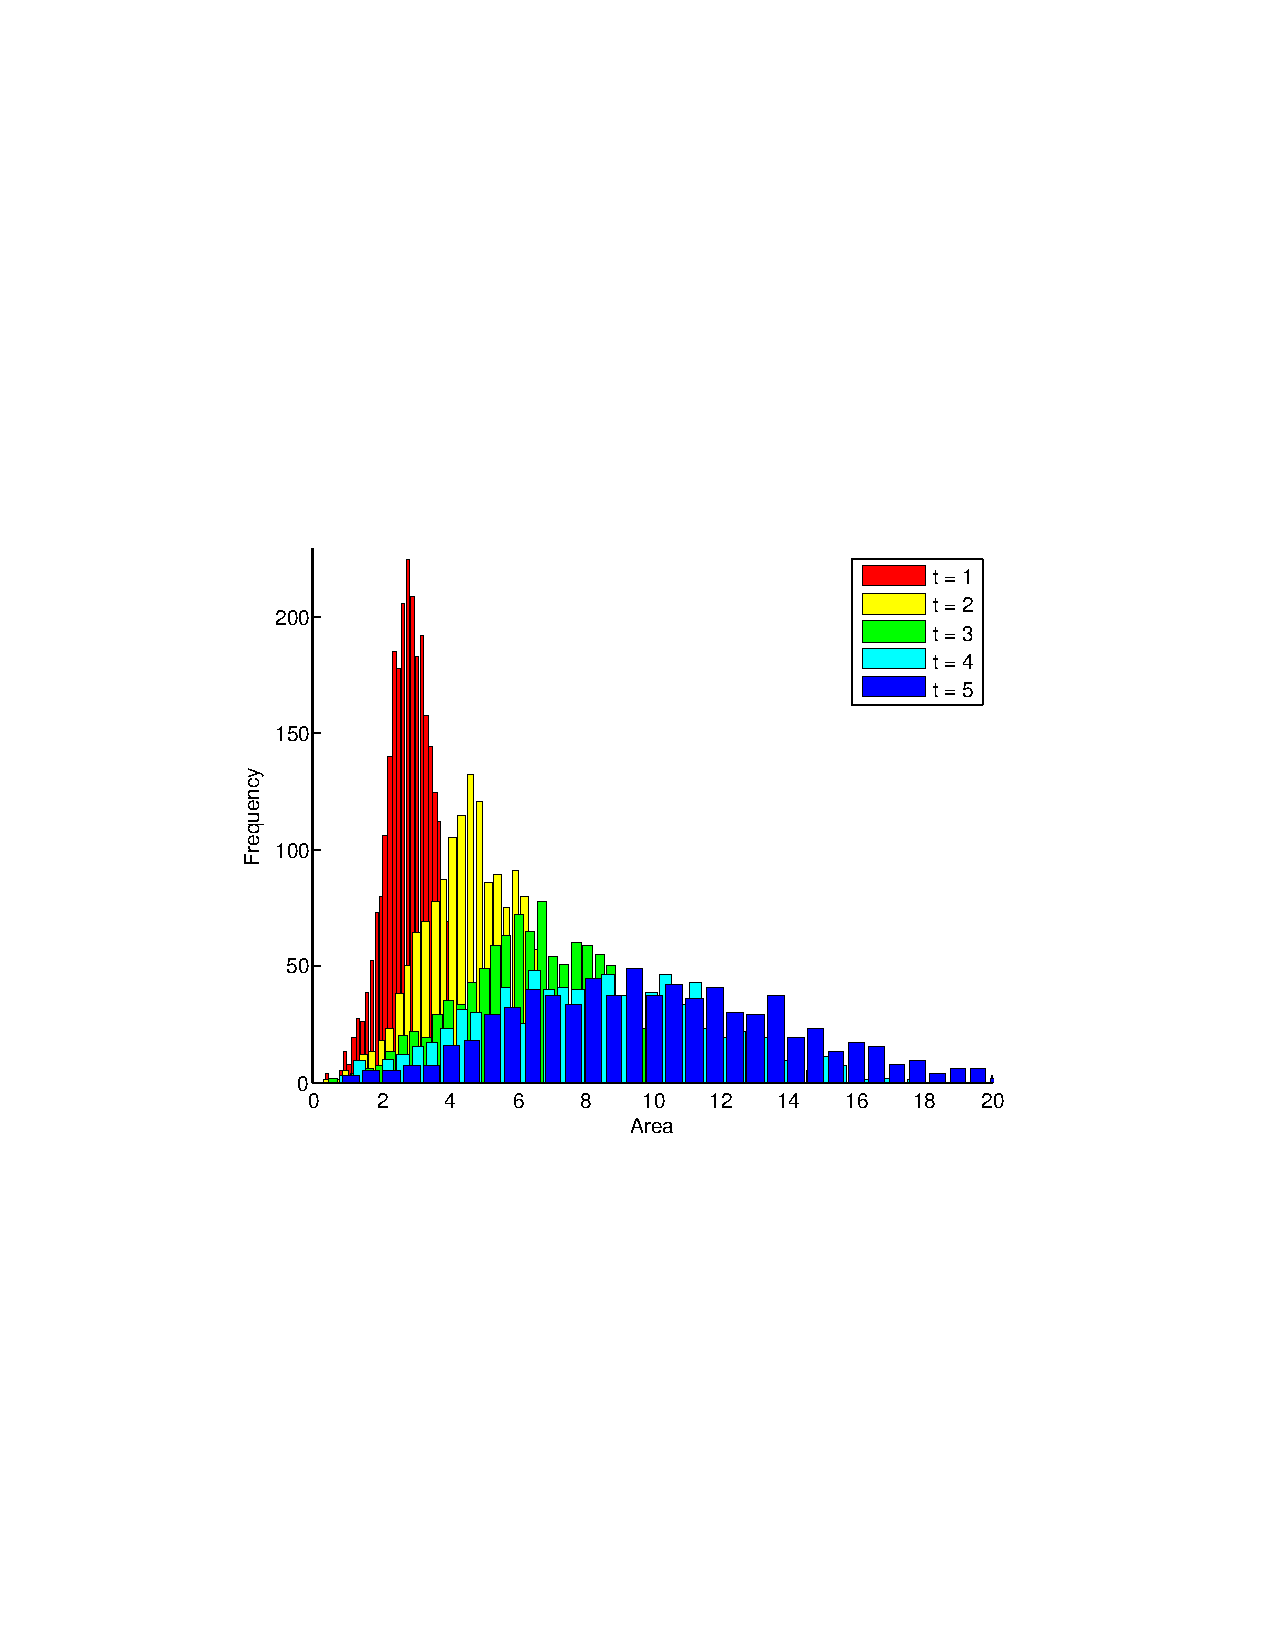
\includegraphics[width=\textwidth]{histbetatenthtier8.pdf}
\vspace{-130pt}
\caption{Histograms of eight-sided grain densities at $\beta = .1$.}
\end{figure}

\begin{figure}
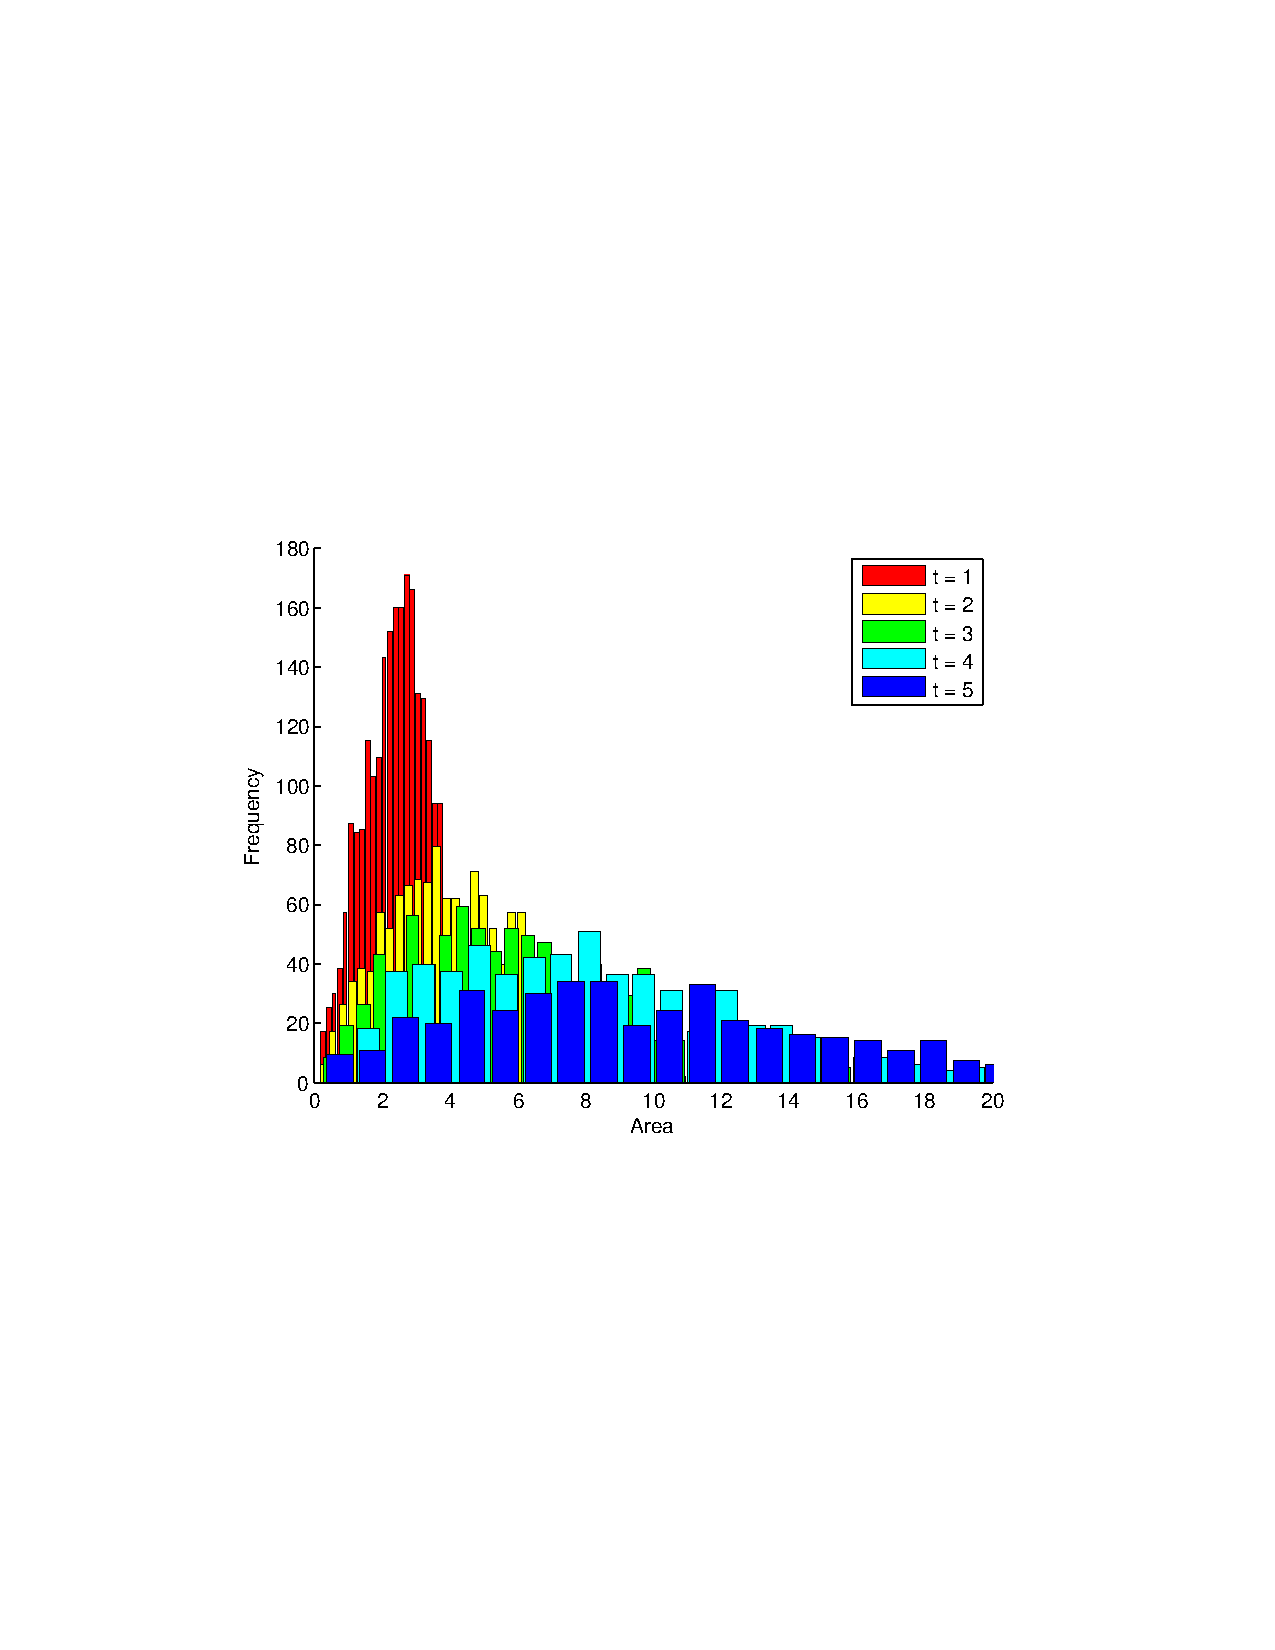
\includegraphics[width=\textwidth]{histbetaonetier8.pdf}
\vspace{-130pt}
\caption{Histograms of eight-sided grain densities at $\beta = 1$.}\label{tierdens9}
\end{figure}

\begin{figure}
\begin{centering}
\includegraphics[width=.5\textwidth]{averageareas.jpg}
\caption{Average areas of grains with sides 2-10 at $\beta= 0$.  Note how for each collection of $n$-gons,for $n= 2, \dots, M$, average area increases linearly.  Similar behavior holds for $\beta= .1$ and $\beta= 1.$}\label{averagewhole}
\end{centering}
\end{figure}

        
\begin{figure}
\centering
        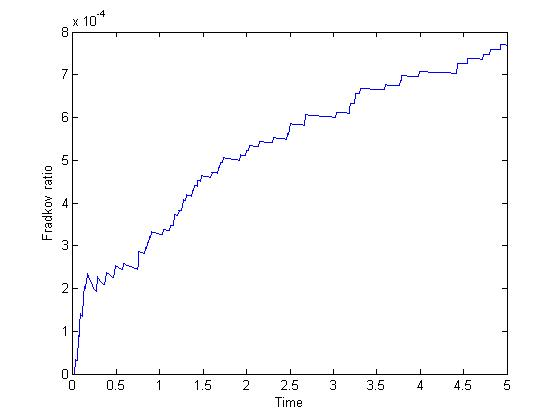
\includegraphics[width=.5\textwidth]{coarseratiobetazero.jpg}
        \caption{Side to grain deletion ratio $\gamma_\beta(t)$ at $\beta=.01$.}\label{fradrat1}
 \end{figure}
       
 \begin{figure}
        \centering
        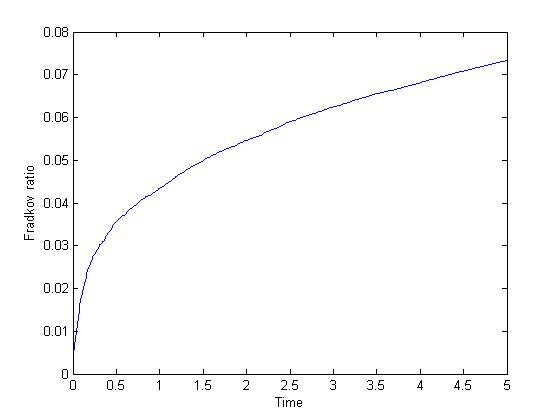
\includegraphics[width=.5\textwidth]{coarseratiobetatenth.jpg}
        \caption{Side to grain deletion ratio $\gamma_\beta(t)$ at $\beta=.1$.}
 \end{figure}       
        
        \begin{figure}
        \centering
        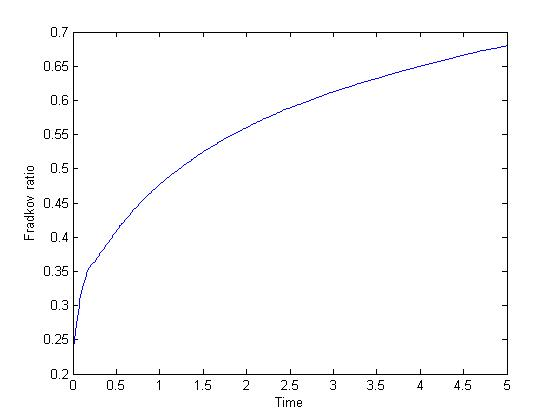
\includegraphics[width=.5\textwidth]{coarseratiobetaone.jpg}
        \caption{Side to grain deletion ratio $\gamma_\beta(t)$ at $\beta=1$.}\label{fradrat3}
       \end{figure}

\clearpage{}

 




